\documentclass[12pt]{article}
\usepackage[english]{babel}
\usepackage[numbers]{natbib}
\usepackage{graphicx}
\usepackage{xcolor}
\usepackage{sectsty}
\usepackage{float}
\bibliographystyle{apalike}
\setcitestyle{open={[},close={]}}
\sectionfont{\color{DarkBlue}} 
\subsectionfont{\color{LightBlue}}
\subsubsectionfont{\color{LightBlue}}
\paragraphfont{\color{LightBlue}}
\subparagraphfont{\color{LightBlue}}
\begin{document}
\definecolor{DarkBlue}{HTML}{4a5a8a} 
\definecolor{LightBlue}{HTML}{4f81bf}
\begin{titlepage}
    \begin{flushleft}
        \vspace{1cm} \Huge  \textbf{Cretaceous Gardens Controller}\\
        \vspace{1cm} \Huge  \textit{Software Requirements Specification}\\
        \vspace{1cm} \Large \textit{SRS Version 2.0}\\
        \vspace{5cm} \LARGE         Team \#3\\ 
                                    05 November 2019
        \vfill       \Huge  \textbf{CS 460 Software Engineering}
    \end{flushleft}
\end{titlepage}
\normalsize \tableofcontents
\pagebreak

\section{Introduction} \label{intro}
\paragraph{} The purpose of this document is to \textit{specify} the requirements for the
development of the Cretaceous Gardens Controller (CGC). The specification is formalized and 
diagrammed in order to guide the eventual implementation of the system. Information 
encountered in the corresponding \textit{Requirements Definition Document} is reiterated 
and restated here where relevant.
      
\paragraph{} After this introduction \footnote{Introduction by Ezequiel Ramos}, 
Section \ref{gen} gives an overview of the system. Section \ref{spec} delves into more 
detail with subsections \ref{logic} and \ref{inter} that feature a more granular view 
of the \textit{Control Logic} and the \textit{External Interfaces}. Section \ref{defs} 
provides the definition of technical terms that will be commonly used.

\section{General Description} \label{gen}
\paragraph{}\textit{This section \footnote{General Description by Siri Khalsa} provides 
a general overview of the whole system. How the system interacts with the hardware interfaces 
and its basic functionality are introduced here. A description of parts to be used in the 
system and the available functionalities for each type are also provided. Some high level 
constraints and assumptions for the system will be also be presented. It should be noted 
that a more detailed specification of constraints is covered in its own section.}
    
    \subsection{Product Perspective}
    \paragraph{} The CGC system as a whole is made up of many smaller subsystems. These systems include cars, T-Rex Monitor, GPS Server, Pay Kiosk, etc. These are clearly defined later in this document primarily in the interfaces section. The CGC is the system that can communicate with everything. The analogy can be used that the CGC is the central nervous system of the entire CGC system. most of the sub-systems will work independent of each other. This is by design. ever system should be able to perform their duties without being affected by the state of another system unless two subsystems are directly interacting. The CGC will get informed that an emergency mode should be triggered from the Electric Fence sub-system. It is the responsibility of the CGC to inform all other sub-systems that we are now in an emergency mode. It is also up to the CGC with the help of an employee to reset everything back into a normal mode of operation.

    \paragraph{} 
    \subsection{Product Functions}
    \paragraph{} The system needs to be maintainable and the redundancy is a central design decision. The CGC itself should be installed on two separate pieces of hardware. Ideally this hardware is located in different physical locations. The secondary location should be located not on the island. This is the recommendation but is not required. The CGC understand the health and status of every subsystem. With the help of human intervention, all components can be be maintained. an example is that the cars can report of their health. If one goes down for whatever reason, the CGC already understand this and helps communicate this information to an employee. The system will automatically deploy a new car (Redundant) to help mitigate the problem while the employees work on permanently fixing the broken car. All sub-systems will have this capability.
    
    \paragraph{} The product will focus on safety. Every decision that is made leads to the safest possible outcome for the visitors and employees. The system is redundant for safety. There are emergency protocols built into every sub-system to guarantee the safest experience possible for all that interact with the CGC system 
        
    \paragraph{} The product will push the limits on the latest technology. The entire system is close to being fully autonomous. The product should feel futuristic and high end. This is a feature designed throughout the components.

    \subsection{User Features}
    \paragraph{} One user feature is the ability to monitor then entire network of nodes as a whole from the CGC Station. The CGC station is a primary interface for employees. It allows employees to help control the system.
        
    \paragraph{} Another feature also available to employees is the ability to interact with the financial aspects of the entire system. This is again performed at the CGC Station where there is a direct connection to the data collected by the CGC System.
        
    \paragraph{} A huge feature of the system is the autonomous behavior of most of the CGC system. The cars pretty much function on their own and most of the other systems do as well. This is a technological advancement that increases the user experience, both visitor and an employee.
    

    \subsection{Assumptions}
    \paragraph{} We assume that the infrastructure is all redundant. The CGC is 
    installed on redundant servers. The network backbone has physical redundant 
    links to appropriate devices like the cameras, the PA speakers, and the 
    electric fence. We will also	program redundancy into the logic. Like the 
    ability to have another car available in case of an emergency or if the car 
    breaks down.

    \paragraph{} Another assumption is that messages would be encrypted in order 
    to provide the security needed, so the messages can not be intercepted and 
    modified.

\section{Specific Requirements} \label{spec}
\paragraph{} \textit{Section Introduction}

    \subsection{External Interfaces} \label{inter}% Anas
    \paragraph{} \textit{The External Interfaces\footnote{External Interfaces by Anas Gauba} 
    make up all the pieces that the CGC communicates with. The CGC itself must 
    communicate with everything, 	but a lot of interfaces can function on their own. The
    car interface is an example of one that needs to be able to function on it's own.}
        
    \paragraph{Pay Kiosk}
    \paragraph {}\textit{The Pay Kiosk interface triggers events in situations where the visitor interaction is required.  }
        \subparagraph{Incoming Events}
        \begin{enumerate}
            \item Register visitor(demographics)/request money.
            \item Accept money(type)/build token.
        \end{enumerate}
                
        \subparagraph{Outgoing Events}
        \begin{enumerate}
            \item Activate token(id).
            \item Dispense token(id). 
            \item Dispense change(money, receipt).
            \item Log transaction. 
            \item Report health status to CGC. 
        \end{enumerate}

    \paragraph{Token}
    \paragraph {}\textit{The events that the Token interface triggers are specifically related to locate the visitor.  }
        \subparagraph{Incoming Events}
        \begin{enumerate}
            \item Trigger Alarm. 
            \item Return to car(carID). 
        \end{enumerate}
                
        \subparagraph{Outgoing Events}
        \begin{enumerate}
            \item Report location to GPS Server(gpsID).
        \end{enumerate}

    \paragraph{Car}
    \paragraph{} \textit{The Car interface triggers events in situations where the visitor interacts with the car as well as the internal sensors that the car is communicating with. }
        \subparagraph{Incoming Events}
        \begin{enumerate}
            \item Read token(tokenID)/Unlock doors or deny access. 
            \item Activate car()[Normal Mode]/Go to south end to pick up visitors.
            \item Activate car()[Emergency Mode]/Go to north end to pick up visitors.
            \item Arrived(Destination)[Normal Mode]/pick up or drop off visitors following the conditioned the protocol.
            \item Arrived(Destination)[Emergency Mode]/pick up or drop off visitors following the conditioned the protocol.
            \item Weight detected.
            \item Change driving mode(modeName).
            \item Activate intercom.
        \end{enumerate}
                
        \subparagraph{Outgoing Events}
        \begin{enumerate}
            \item The GPS current location(id).
            \item Alert visitors(carID).
            \item Trigger alarm.
            \item Report health status to CGC.
        \end{enumerate}

    \paragraph{T-Rex Monitor}
    \paragraph{}\textit{The T-Rex Monitor interface triggers events in situations where 
    the actions of T Rex can be monitored appropriately. }
        \subparagraph{Incoming Events}
        \begin{enumerate}
            \item Inject tranquilizer. 
        \end{enumerate}
                
        \subparagraph{Outgoing Events}
        \begin{enumerate}
            \item Report T-Rex health.
            \item Report health status to CGC.
            \item Report location to GPS Server(gpsID).
        \end{enumerate}

    \paragraph{Camera Network}
    \paragraph{}\textit{The Camera Network interface triggers events in situations 
    where each specific cameras operations can be easily monitored. }
        \subparagraph{Incoming Events}
        \begin{enumerate}
            \item Delete recording(cameraID, date range).
            \item Activate recording(cameraID).
            \item Monitor streaming(cameraID).
        \end{enumerate}
        
        \subparagraph{Outgoing Events}
        \begin{enumerate}
            \item Camera outage(cameraID).
            \item Report health status to CGC. 
        \end{enumerate}

    \paragraph{Electric Fence}
    \paragraph{}\textit{The Electric Fence interface triggers events in the case of any possible distortion in the panels. }
        \subparagraph{Incoming Events}
        \begin{enumerate}
            \item Null.
        \end{enumerate}
                
        \subparagraph{Outgoing Events}
        \begin{enumerate}
            \item Electricity distortion/trigger an emergency mode.
            \item Report health status to CGC. 
        \end{enumerate}

    \paragraph{Global Alarm System}
    \paragraph{}\textit{The Global Alarm System interface triggers events in situations whenever 
    there are announcements to be made all across the park. }
        \subparagraph{Incoming Events}
        \begin{enumerate}
            \item Trigger alarms[Emergency Mode]/play emergency alarm sound.
            \item Trigger alarms[Normal Mode]/play Public Service Announcement (PSA).
            \item Disable alarms.
        \end{enumerate}
                
        \subparagraph{Outgoing Events}
        \begin{enumerate}
            \item Report health status to CGC.
        \end{enumerate}

    \paragraph{CGC Station}
    \paragraph{}\textit{The CGC Station interface triggers events in situations where an employee has to respond in specific situations. }
        \subparagraph{Incoming Events}
        \begin{enumerate}
            \item Review health status of all the associated devices.
        \end{enumerate}
                
        \subparagraph{Outgoing Events}
        \begin{enumerate}
            \item Activate tranquilizer.
            \item Deactivate emergency mode.
            \item Activate intercom. 
        \end{enumerate}

    \paragraph{GPS Server}
    \paragraph{}\textit{The GPS Server interface triggers events in situations of tracking the GPS devices. }
        \subparagraph{Incoming Events}
        \begin{enumerate}
            \item Track location(gpsID).
        \end{enumerate}
                
        \subparagraph{Outgoing Events}
        \begin{enumerate}
            \item Report location(gpsID).
        \end{enumerate}						
        
    \subsection{Control Logic} \label{logic}%siri
    \paragraph{} \textit{ This section outlines the control logic of the CGC system. Due to the size of the entire system we have broken down the logic diagrams into the sub-components of the CGC\footnote{Control Logic by Siri Khalsa, Anas Gauba and Santi}
    The explanation for each component can be seen below. The Control Logic diagram for the CGC system as a whole was missed due to time constraints but is planned to be added in the future if time permits.}

    \paragraph{Pay Kiosk}
    \paragraph{}\textit{The Pay Kiosk logic can be seen below. the goal is to help communicate with potential visitors and help them purchase tokens to gain access to the garden.
    The system starts at the main screen and will move into separate states to help facilitate the sale. If the emergency mode is triggered in the CGC system than the Pay kiosk will return the the main screen.}
    \begin{figure}[H]
         \centerline{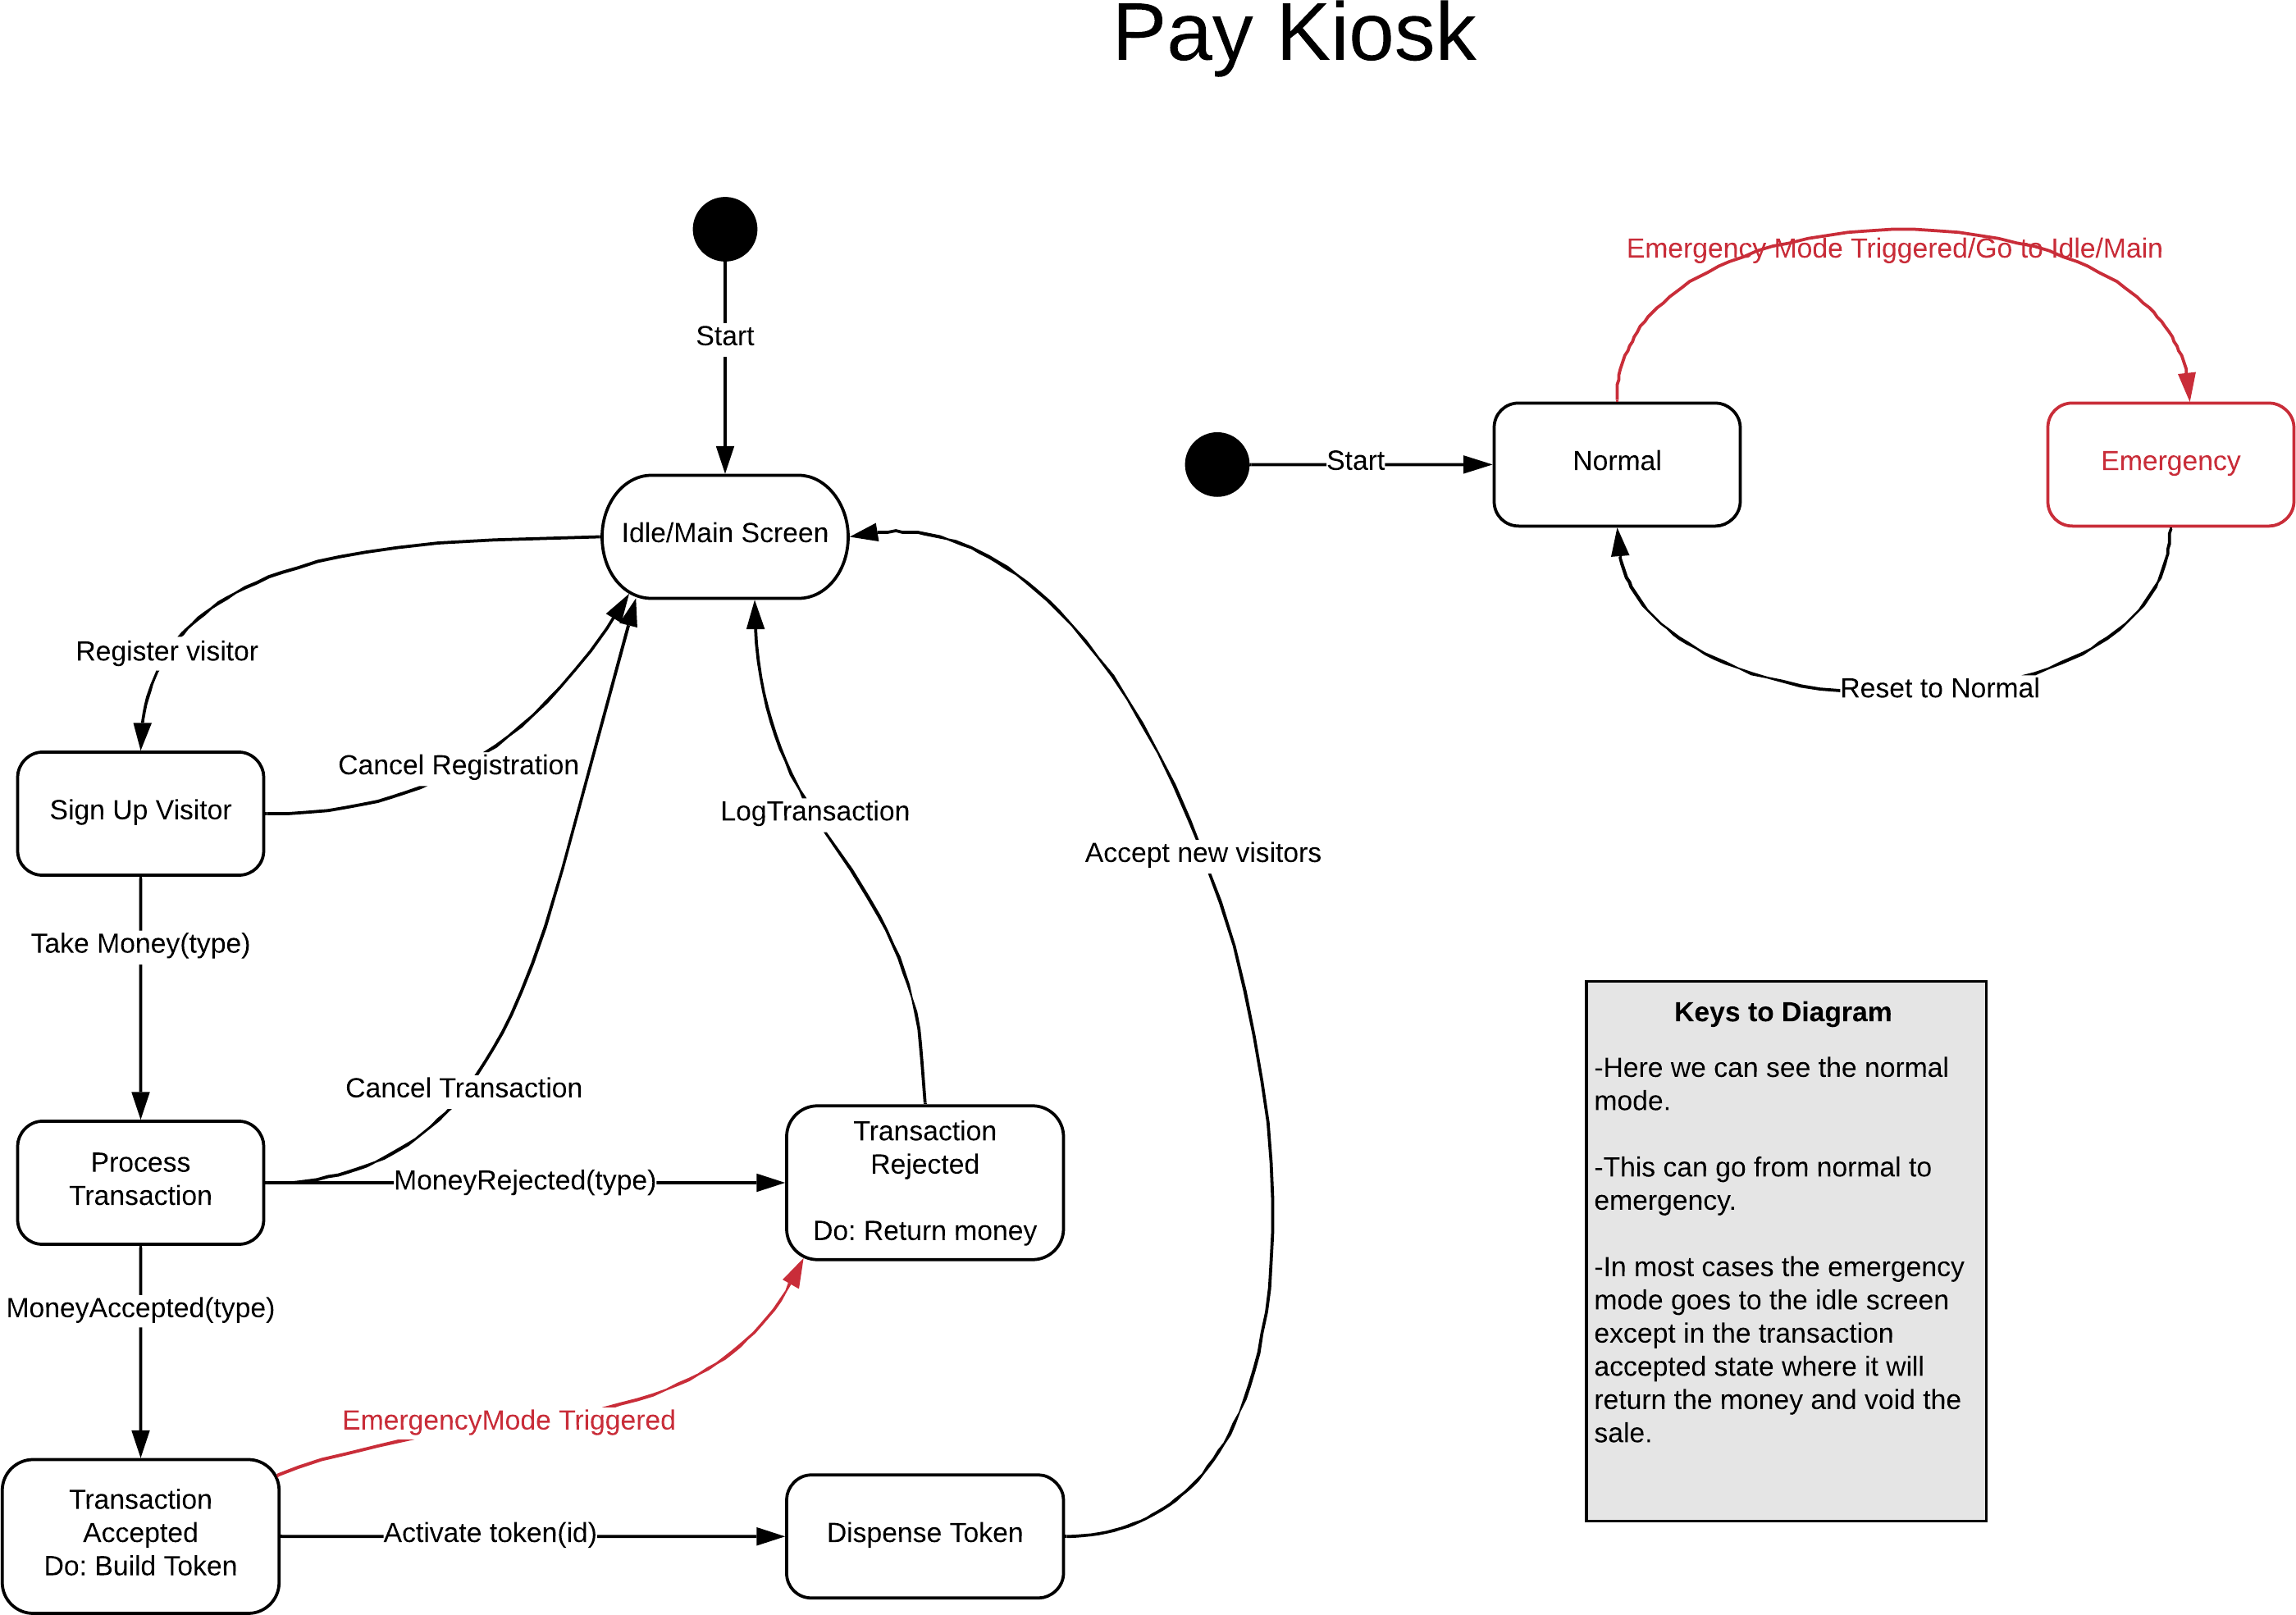
\includegraphics[scale=0.70]{PayKiosk.png}}
         \caption{Pay Kiosk Dynamic Control Model}
          \label{fig:paykiosk}
    \end{figure}

    \paragraph{Token}
    \paragraph{}\textit{The Tokens logic is extremely simple. It is in an activated state when deployed to a visitor. Here it will perform all of its functions. The GPS will send signals to the GPS server. It will also sound an alarm or display and sound information.}
    \begin{figure}[H]
         {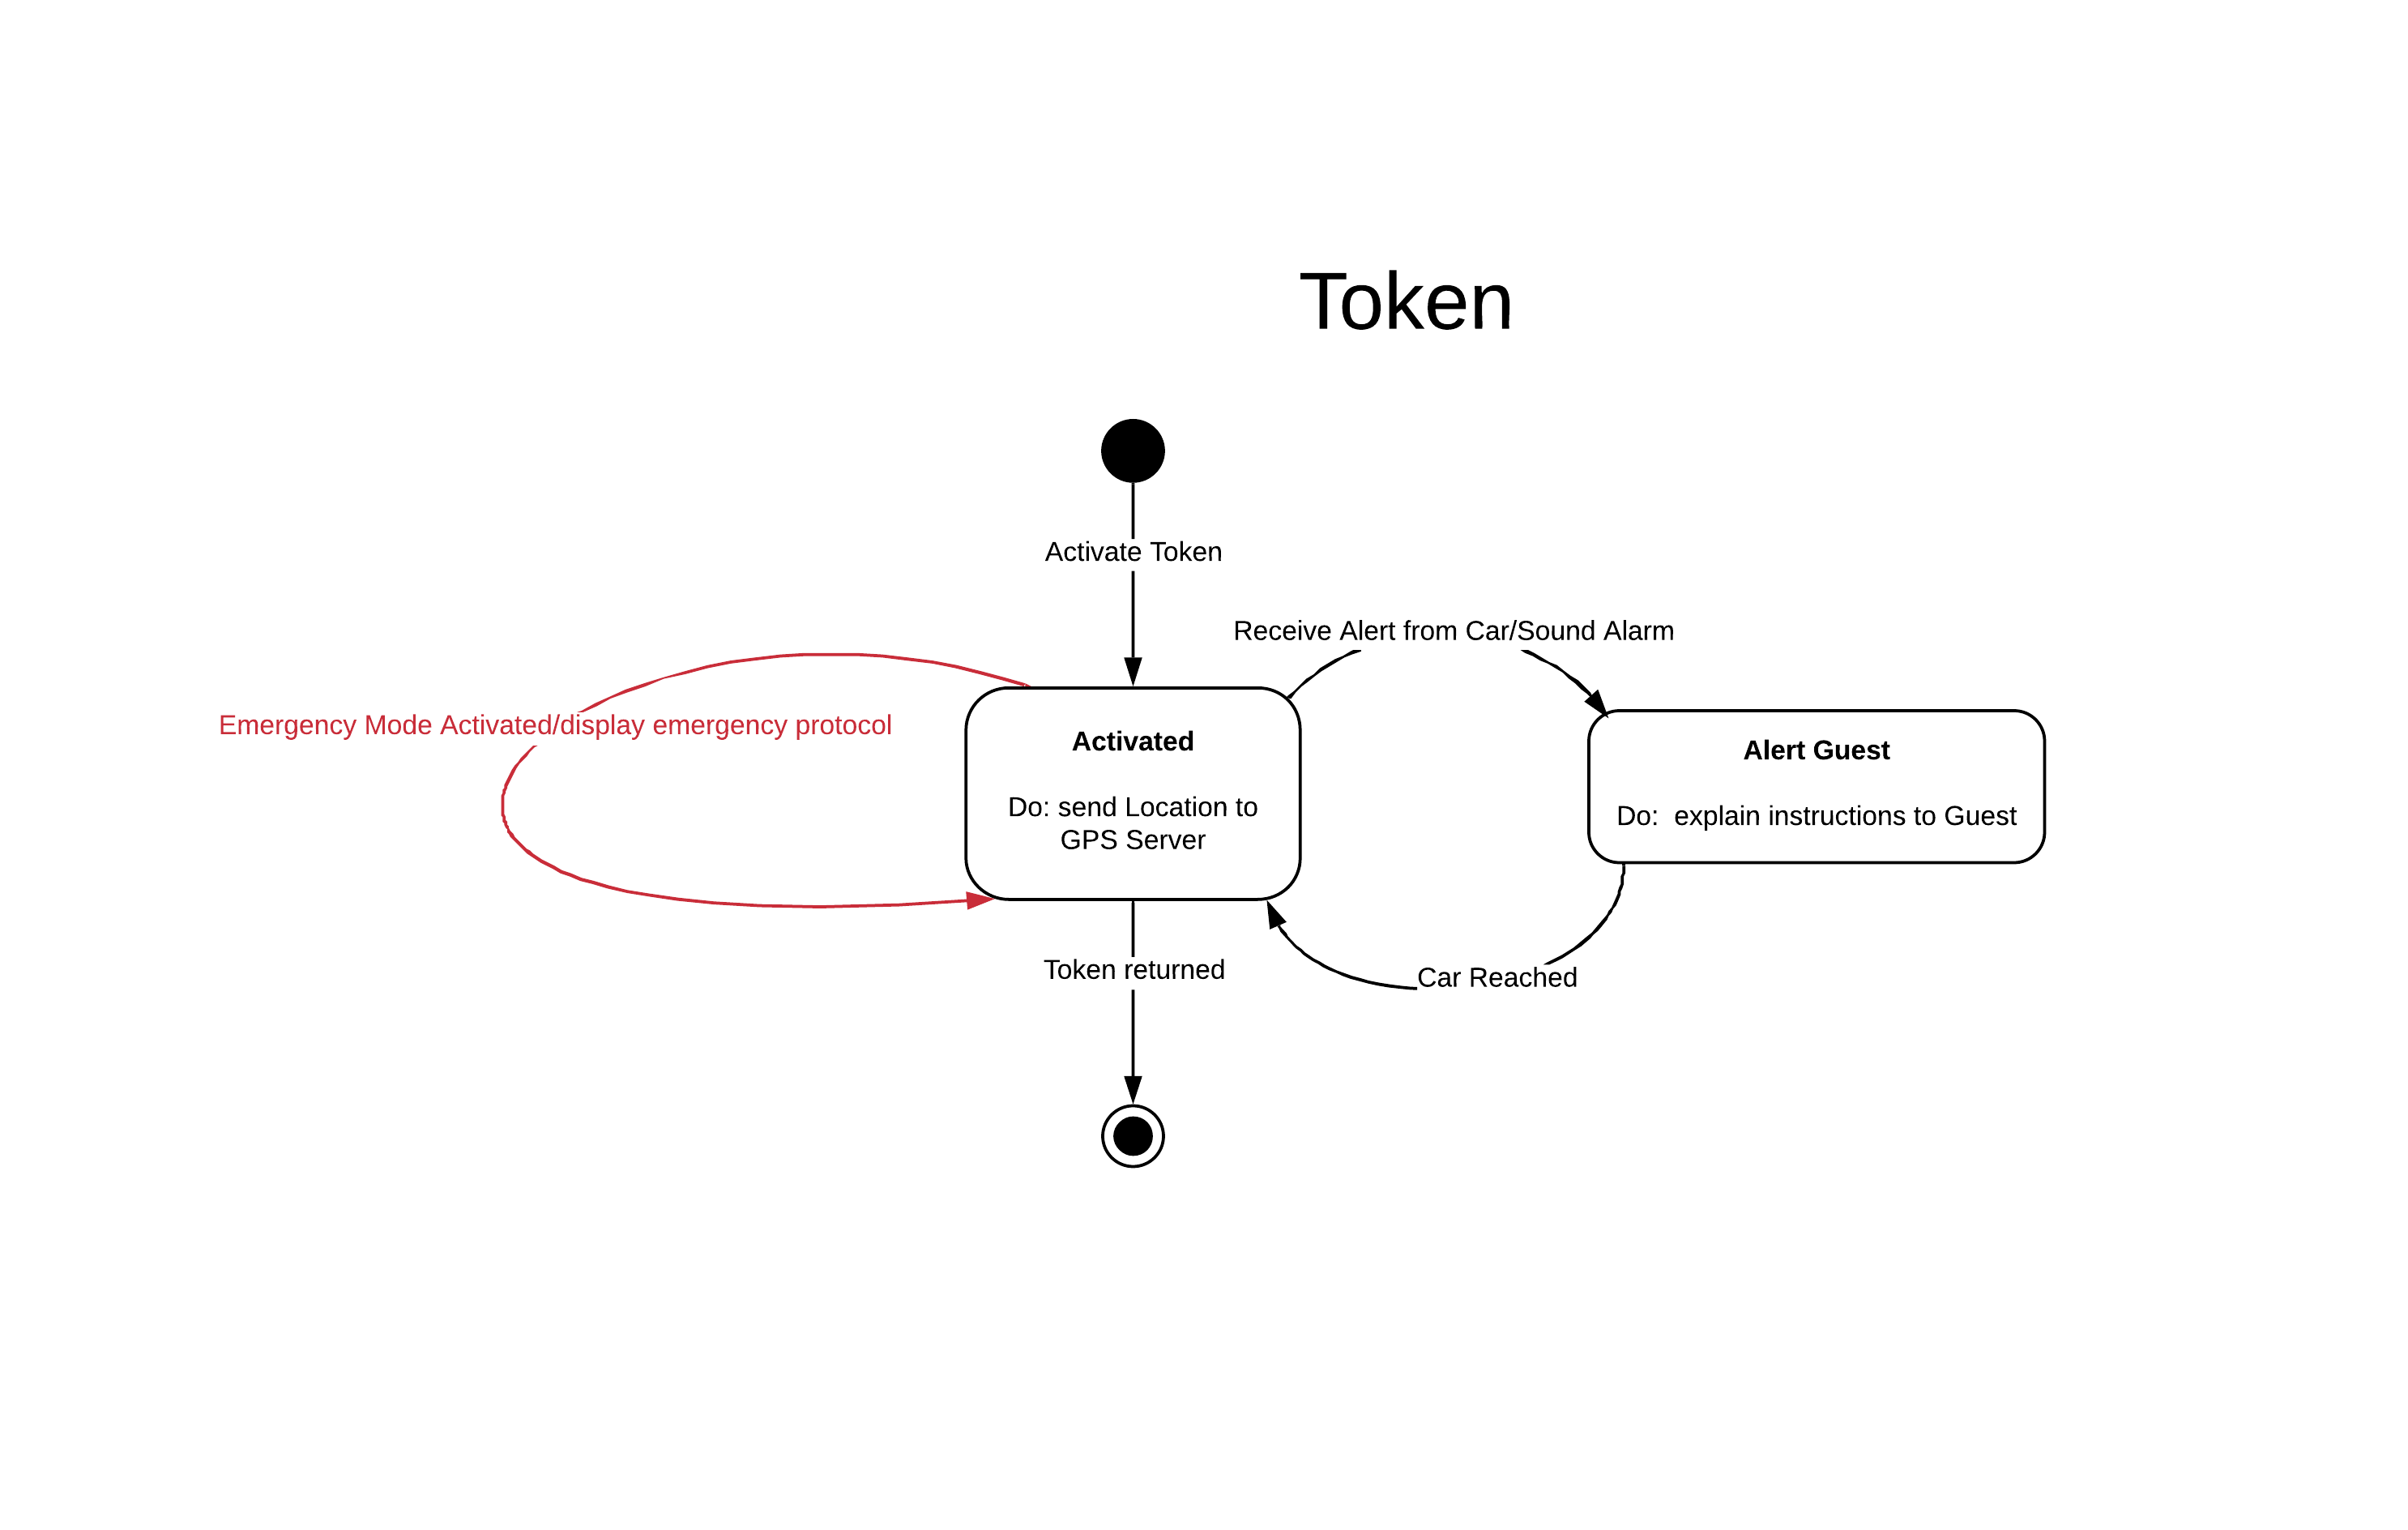
\includegraphics[scale=0.80]{Token.png}}
         \caption{Token Dynamic Control Model}
          \label{fig:token}
    \end{figure}

    \paragraph{CGC Station}
    \paragraph{}\textit{This is one of the more complex subsystems. The logic here states that there are separate screens that act as states. The main screen displays access to other screens 
    and a general overview of the state of everything connected to the CGC. This system can change states to screens such as the Health Status screen, which can display the health status of all reporting devices.
    Another screen that can be accessed is the Emergency screen here all actions related to controlling the CGC when the emergency mode has been activated can be seen. The same type of logic can be inferred through out the rest of the screens which are made available.}
    \begin{figure}[H]
         \centerline{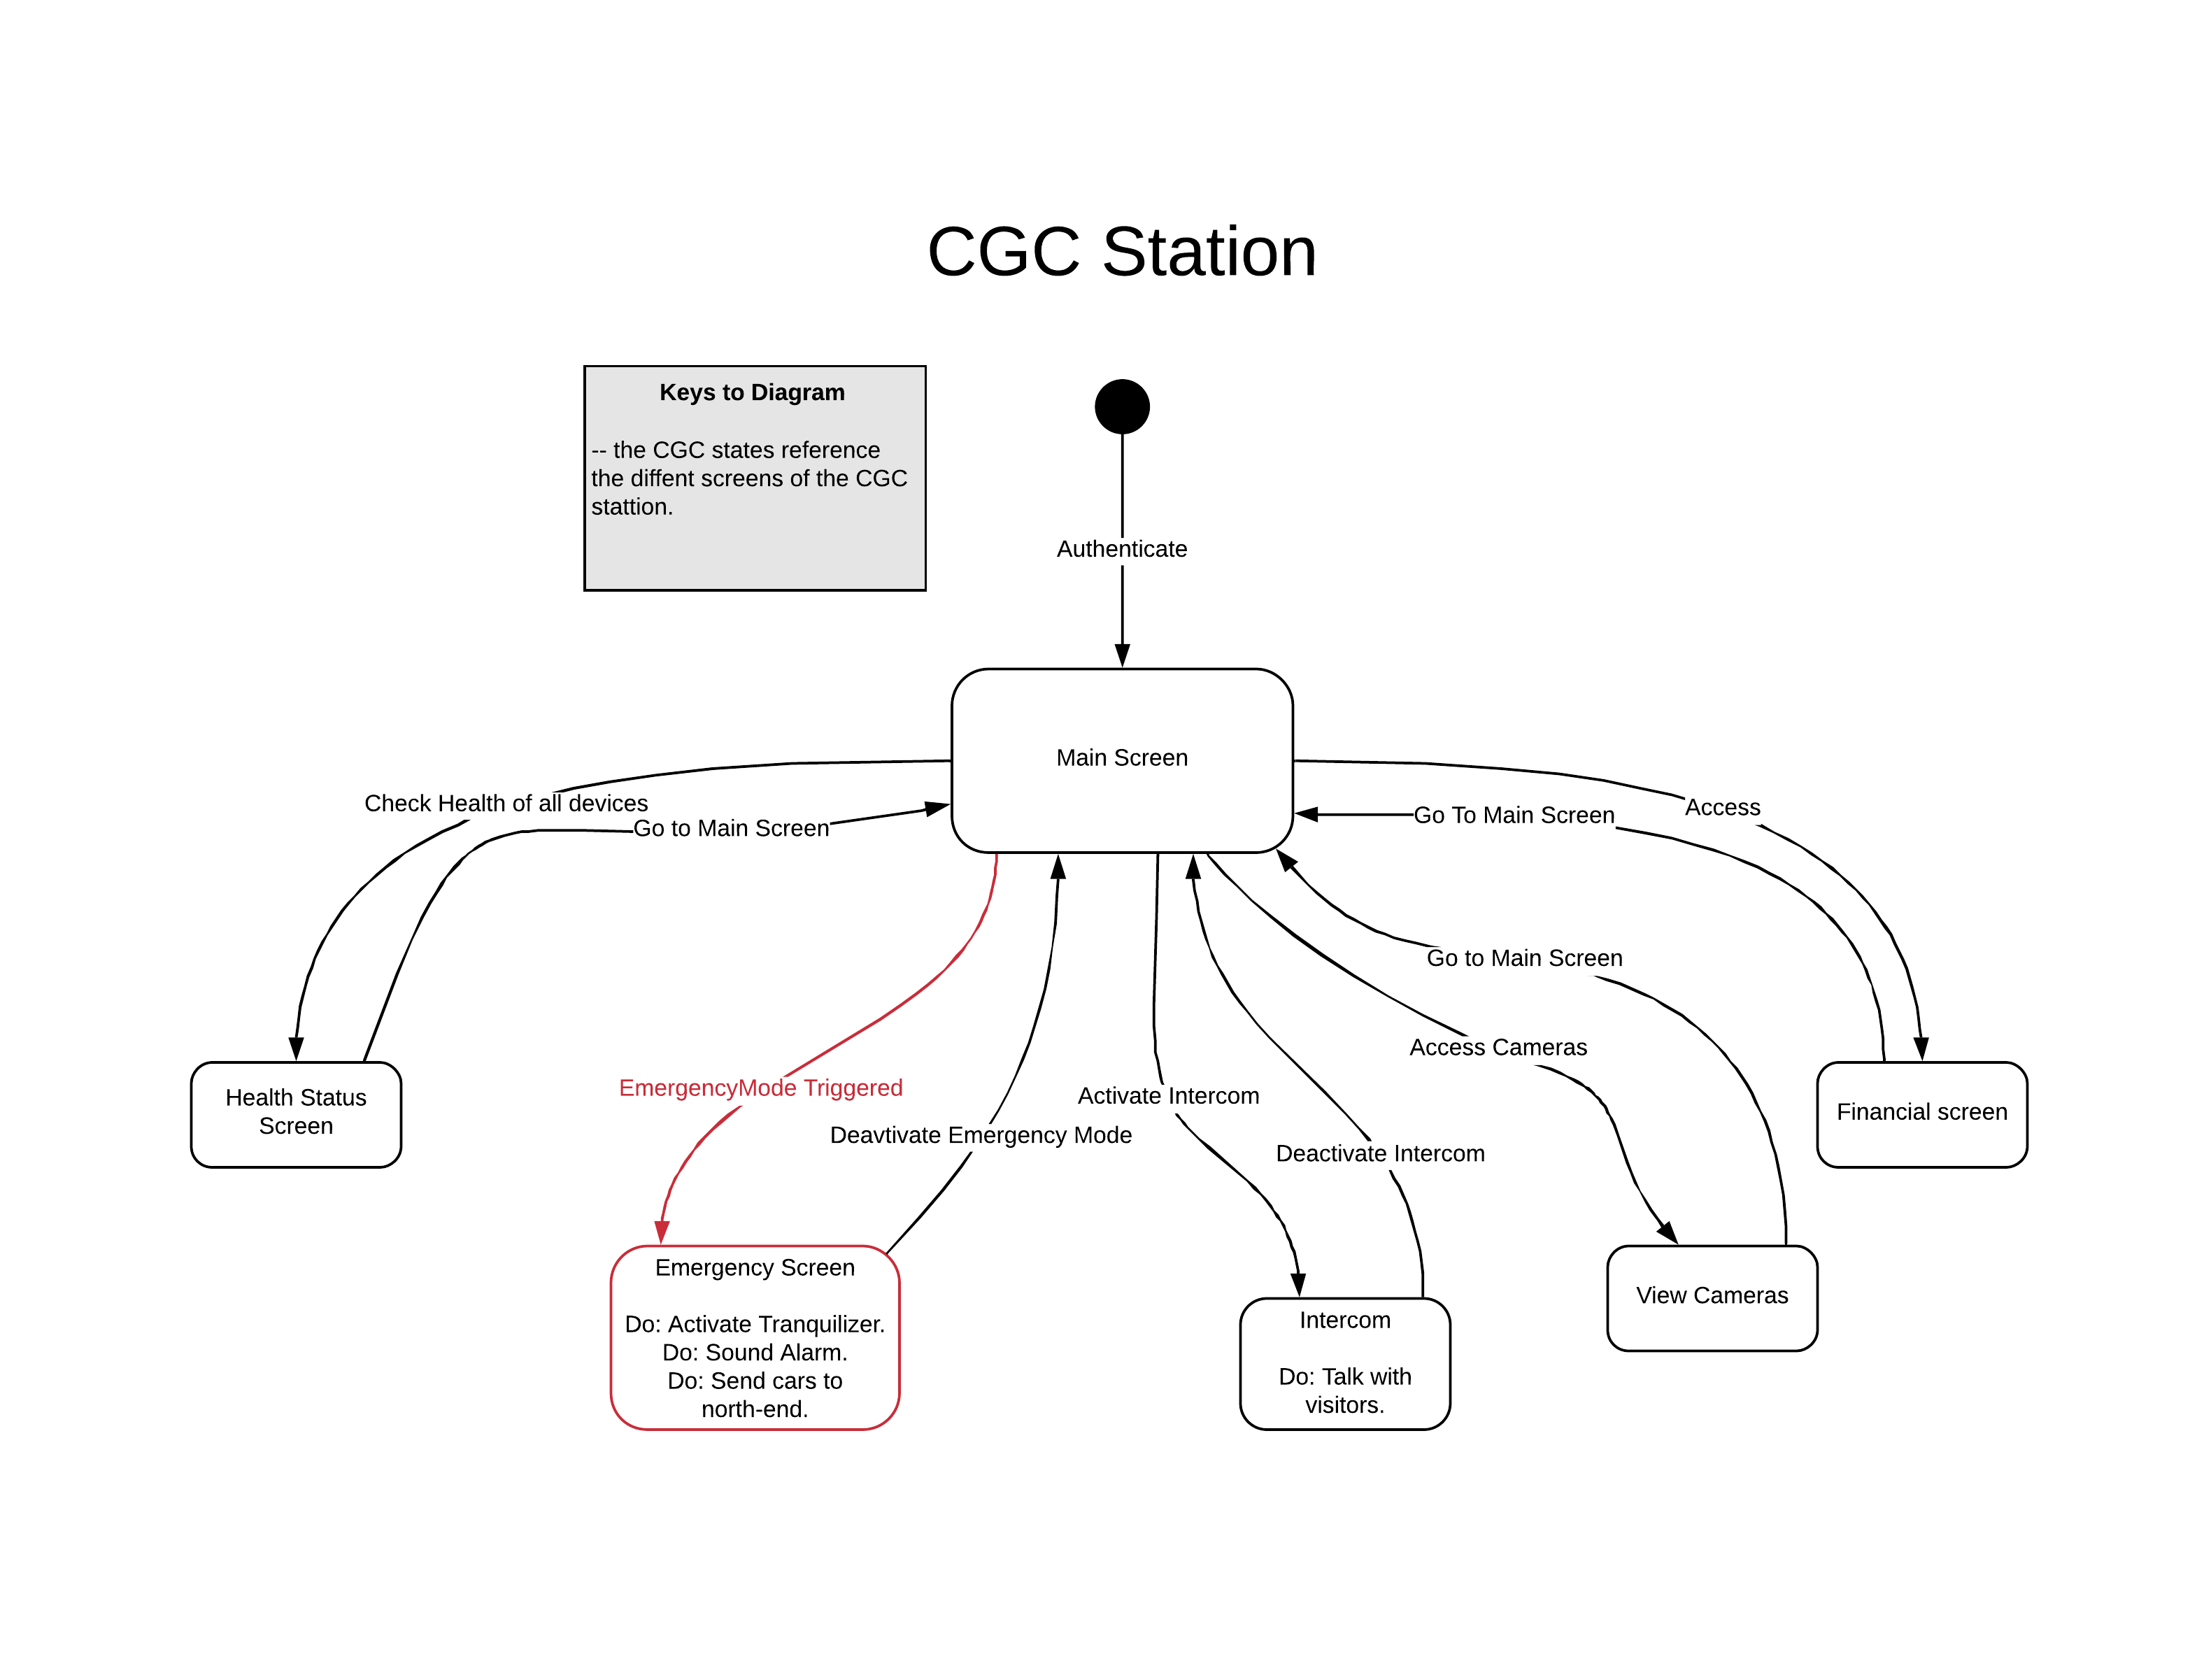
\includegraphics[scale=0.80]{CGCStation.png}}
         \caption{CGC Station Dynamic Control Model}
          \label{fig:cgcstation}
    \end{figure}

    \paragraph{Car Normal Mode}
    \paragraph{}\textit{The car is incredibly complex. To successfully explain the Car logic two diagrams were created. This diagram is for the Normal mode of the car. There are some main states that the car is in. All cars start out in an inactive state where they wait to be activated. In the case of
    this diagram they will be activated with the goal of picking up visitors at the south end of the island. They move immediately into the Drive to South state. This is a state that implies the car is actively drive with the destination of the South end.
    When the car arrives at the destination is always going into a drop off state. when ready for passengers it will move into a pick up state. There is another state of Driving to North End. If the car drops off after this destination, It will go to a waiting state while the visitors it brought over enjoy the exhibit.}
    \begin{figure}[H]
         \centerline{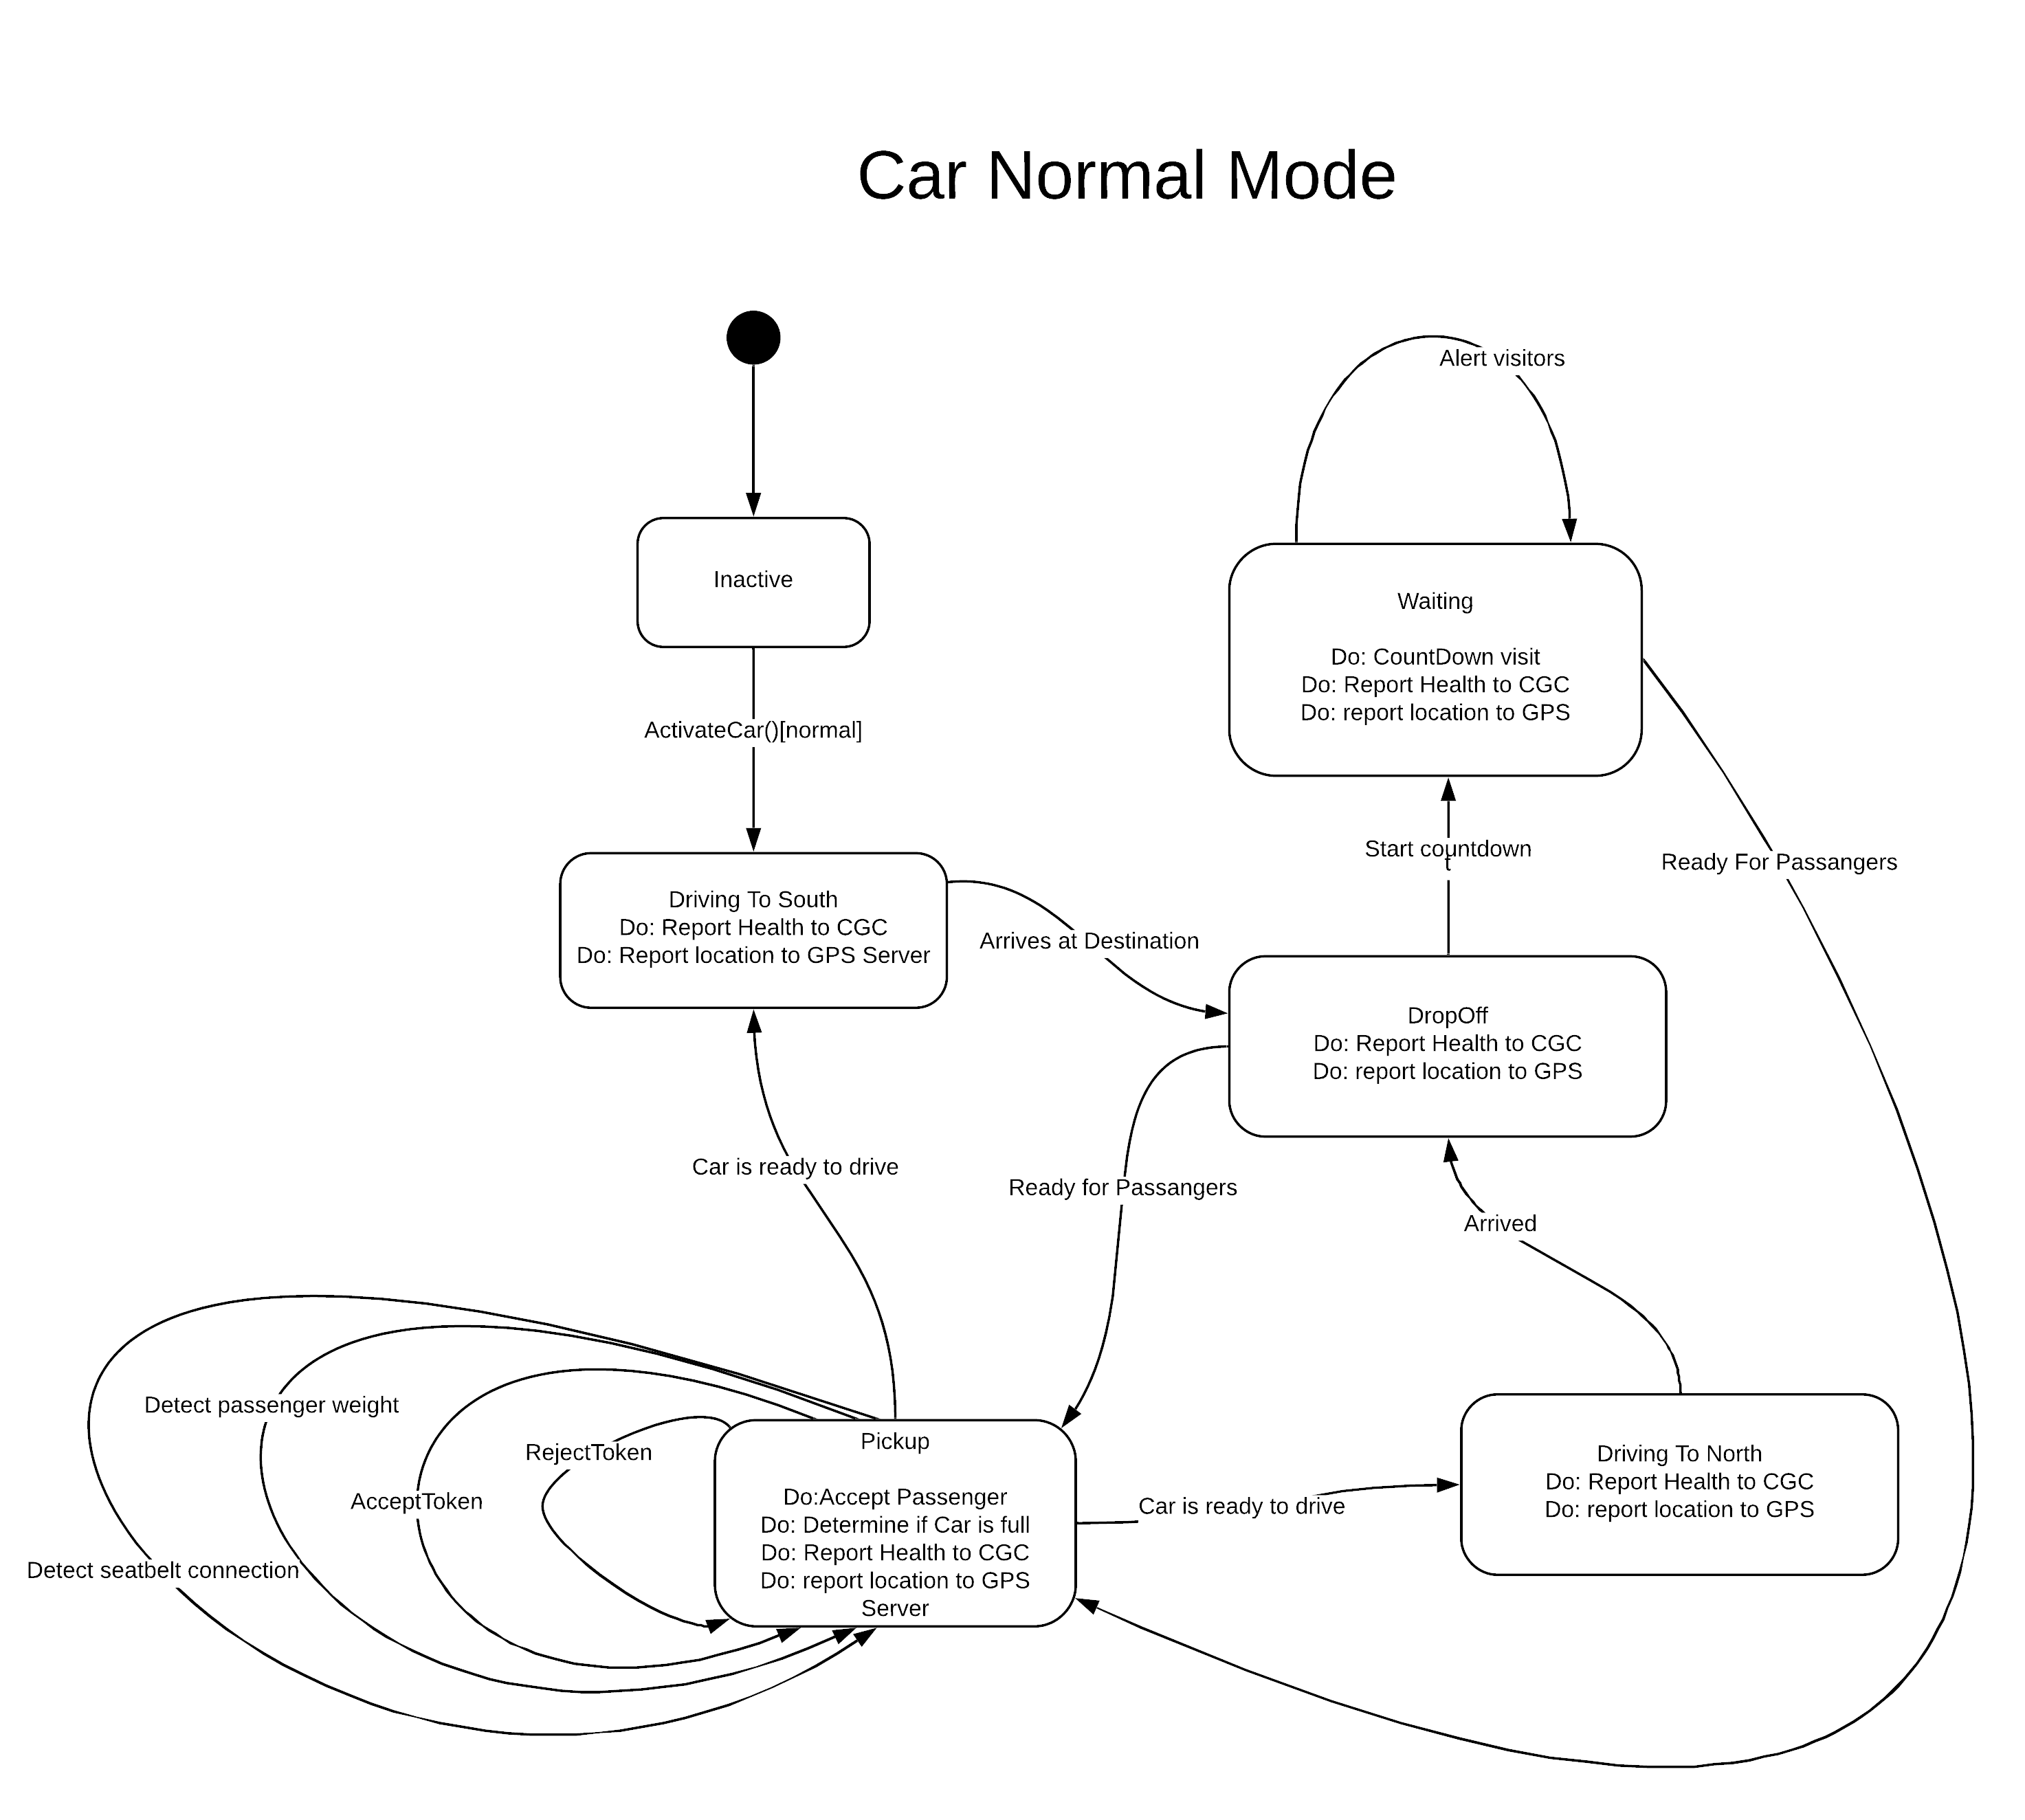
\includegraphics[scale=0.60]{CarNormalMode.png}}
         \caption{Car Normal Mode Dynamic Control Model}
          \label{fig:carnormalmode}
    \end{figure}

    \paragraph{Car Emergency Mode}
    \paragraph{}\textit{This is the second diagram for the car. It explains the logic the car follows inside of an emergency triggered state. All spare cars drive to the north end. they pick up passengers and move back to the south end.}
    \begin{figure}[H]
         \centerline{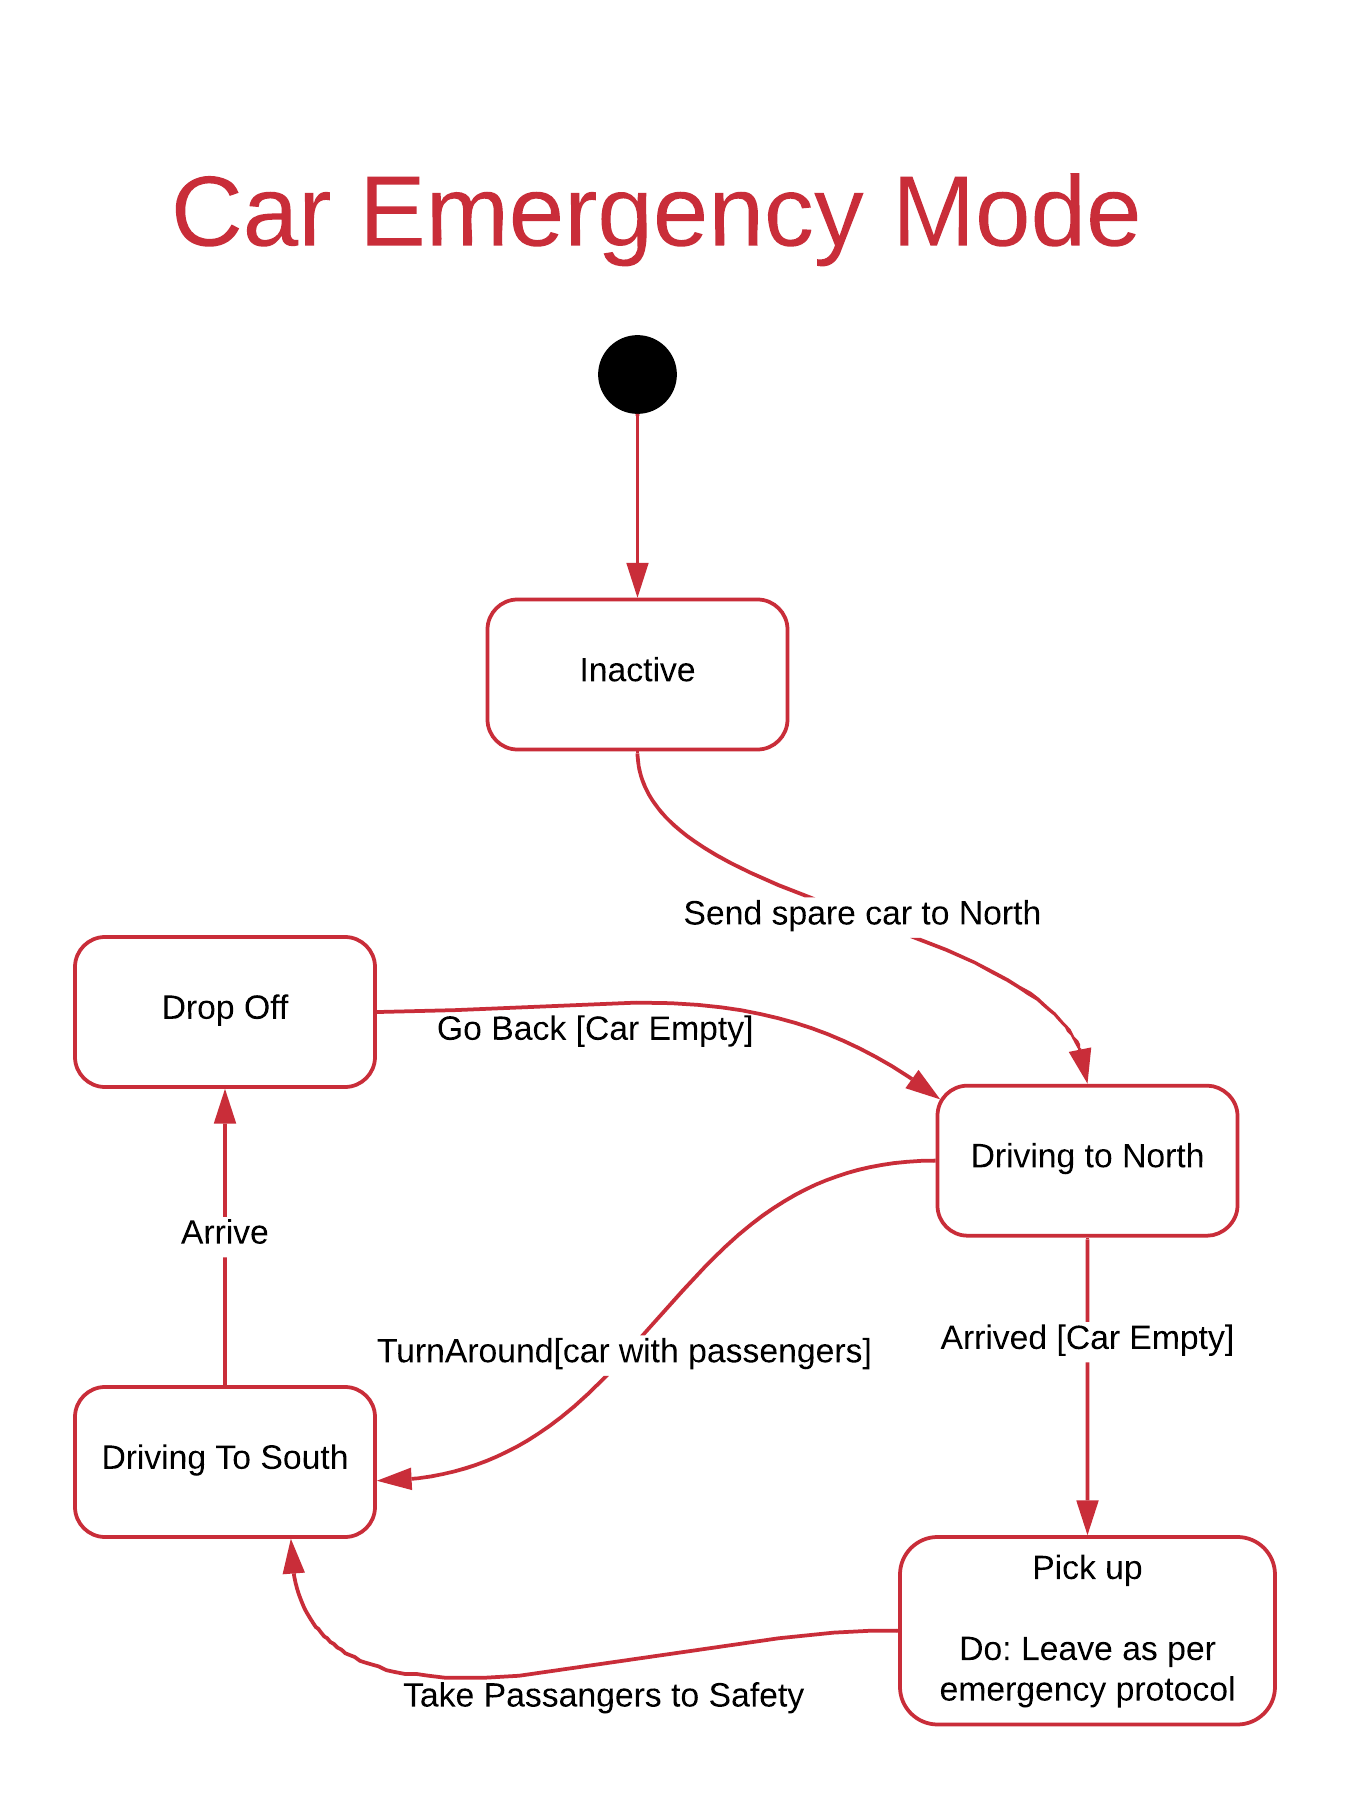
\includegraphics[scale=0.80]{CarEmergencyMode.png}}
         \caption{Car Emergency Mode Dynamic Control Model}
          \label{fig:caremergencymode}
    \end{figure}

    \paragraph{GPS Server}
    \paragraph{}\textit{The Control Logic for the GPS server is very simple the system is either in a healthy state where all nodes are healthy and accounted for and the system itself is running healthy. The other state is a degraded state. This state includes a down GPS client or a down GPS server.}
    \begin{figure}[H]
         \centerline{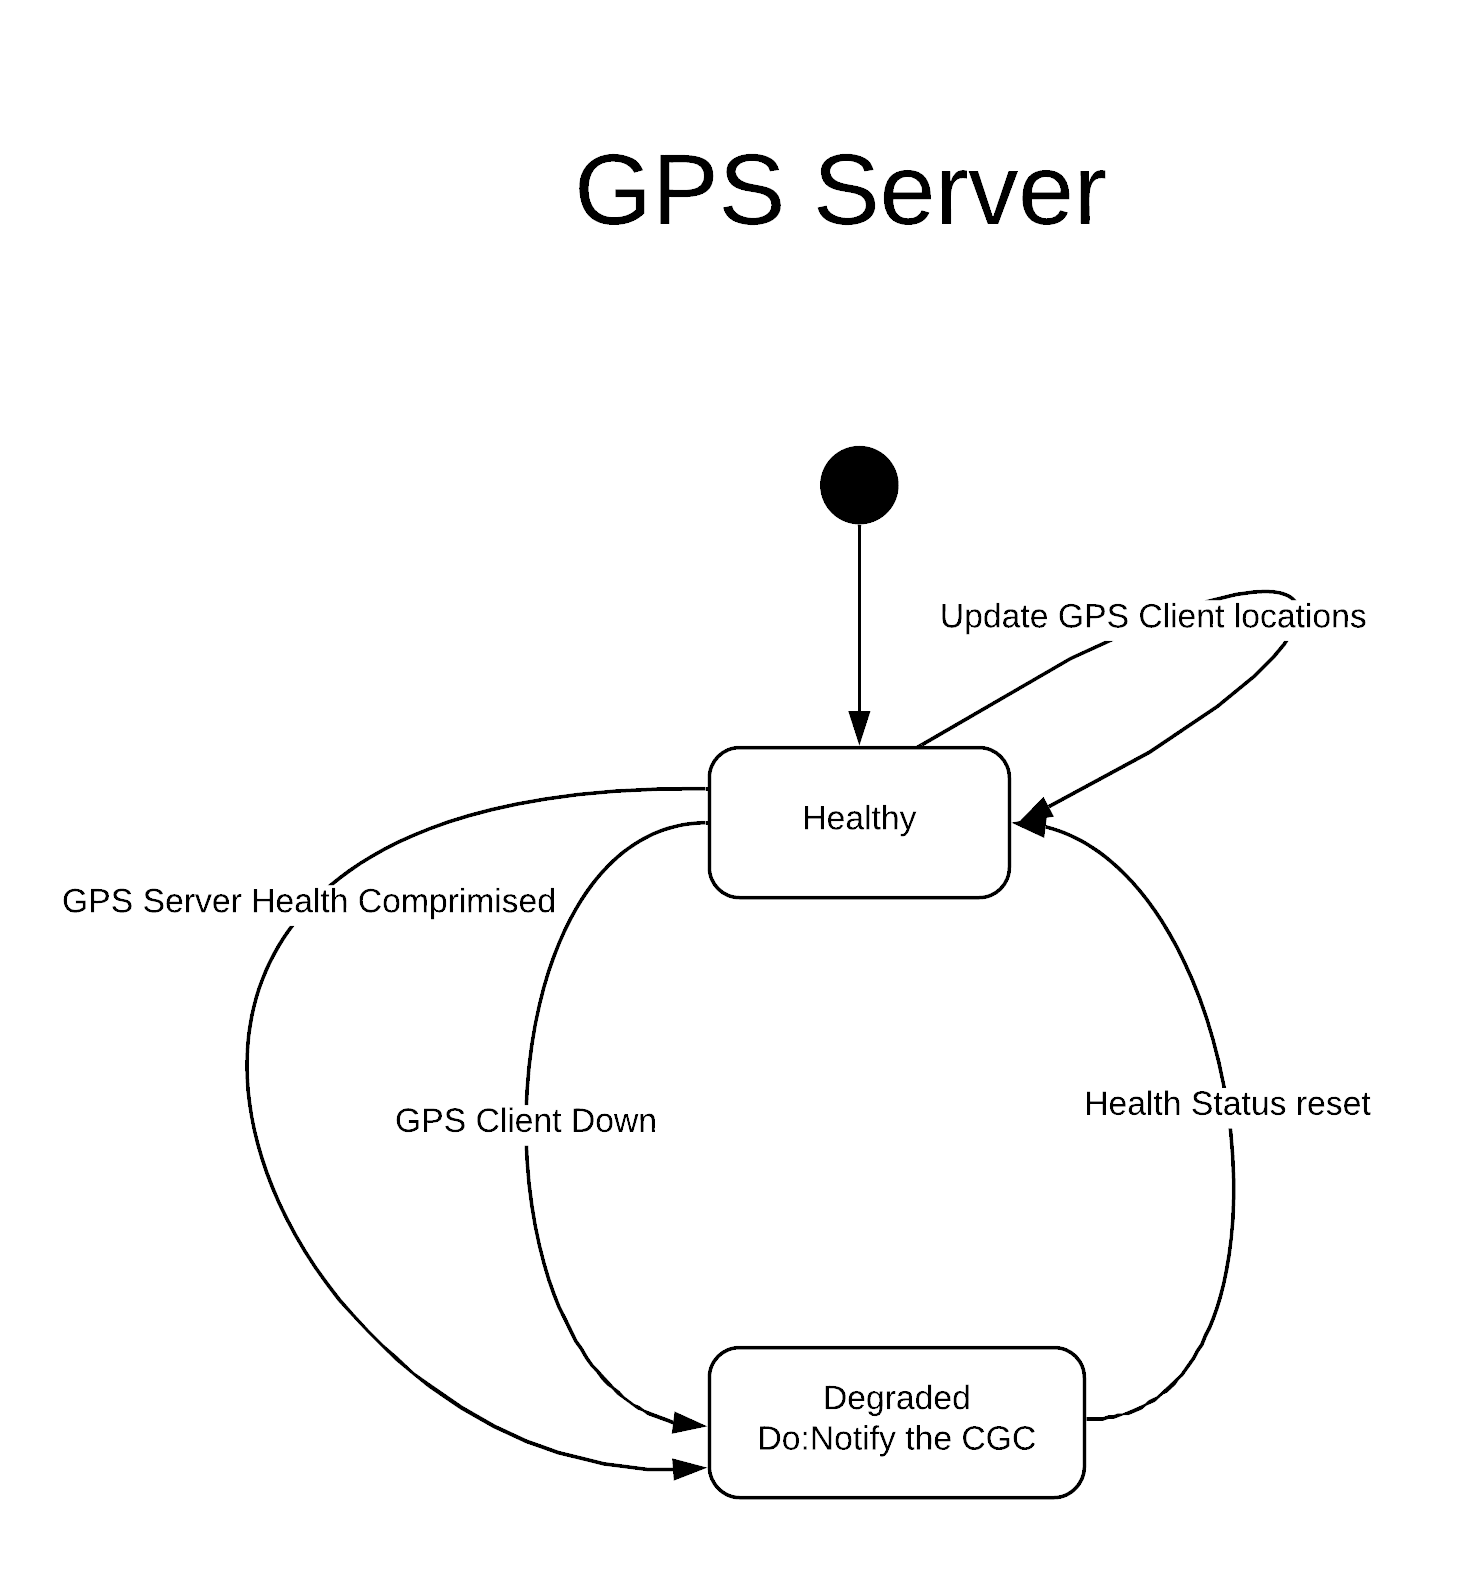
\includegraphics[scale=0.80]{GPSServer.png}}
         \caption{GPS Server Dynamic Control Model}
          \label{fig:gpsserver}
    \end{figure}

    \paragraph{Global Alarm System}
    \paragraph{}\textit{The Global Alarm System logic is also very simple. the speakers can either be active and doing something or the system can be idle waiting to be triggered into an active state.}
    \begin{figure}[H]
         \centerline{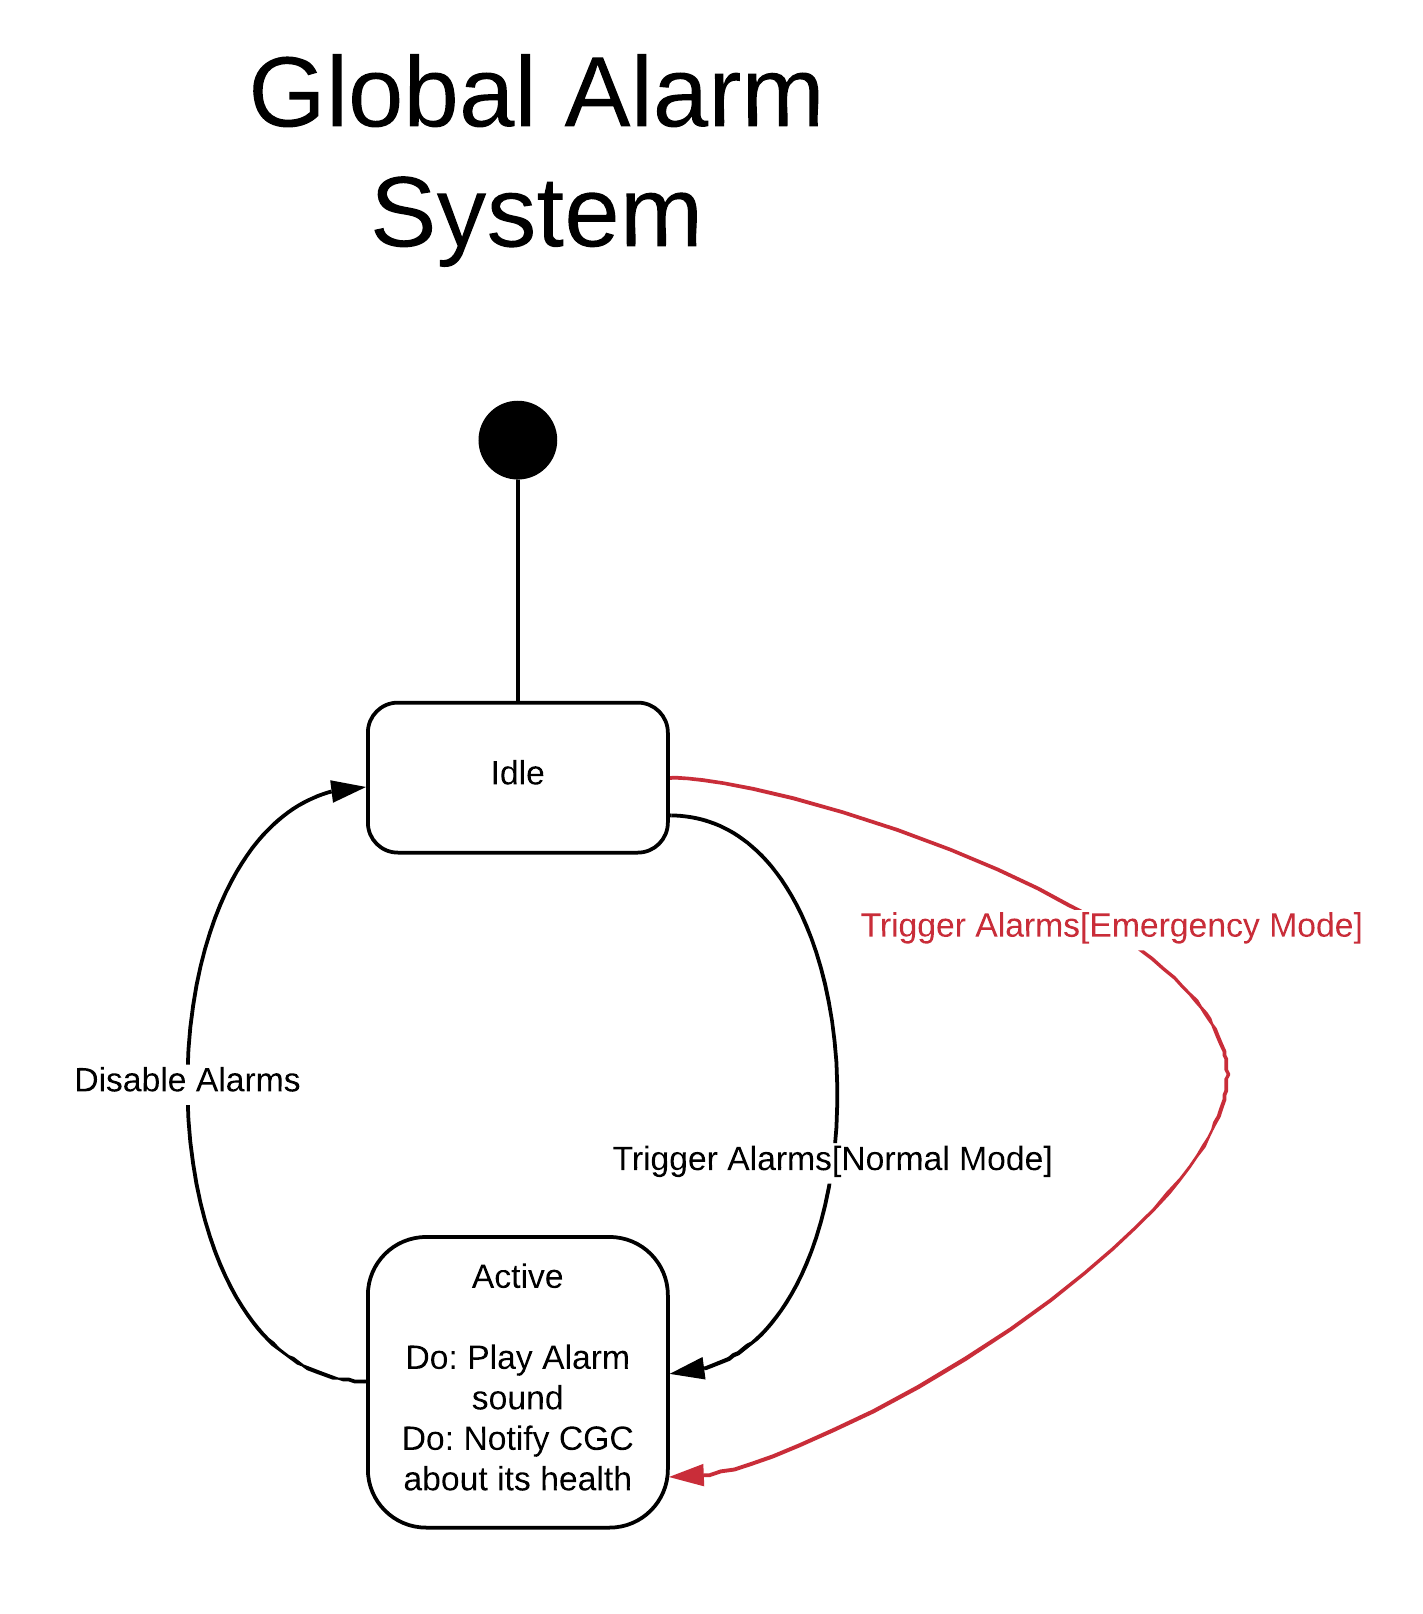
\includegraphics[scale=0.80]{GlobalAlarmSystem.png}}
         \caption{Global Alarm System Dynamic Control Model}
          \label{fig:globalalarmsystem}
    \end{figure}

    \paragraph{Camera Network}
    \paragraph{}\textit{The camera network has a healthy state and degraded state. it also has a DVR state where the system can manage recordings of video feeds.}
    \begin{figure}[H]
         \centerline{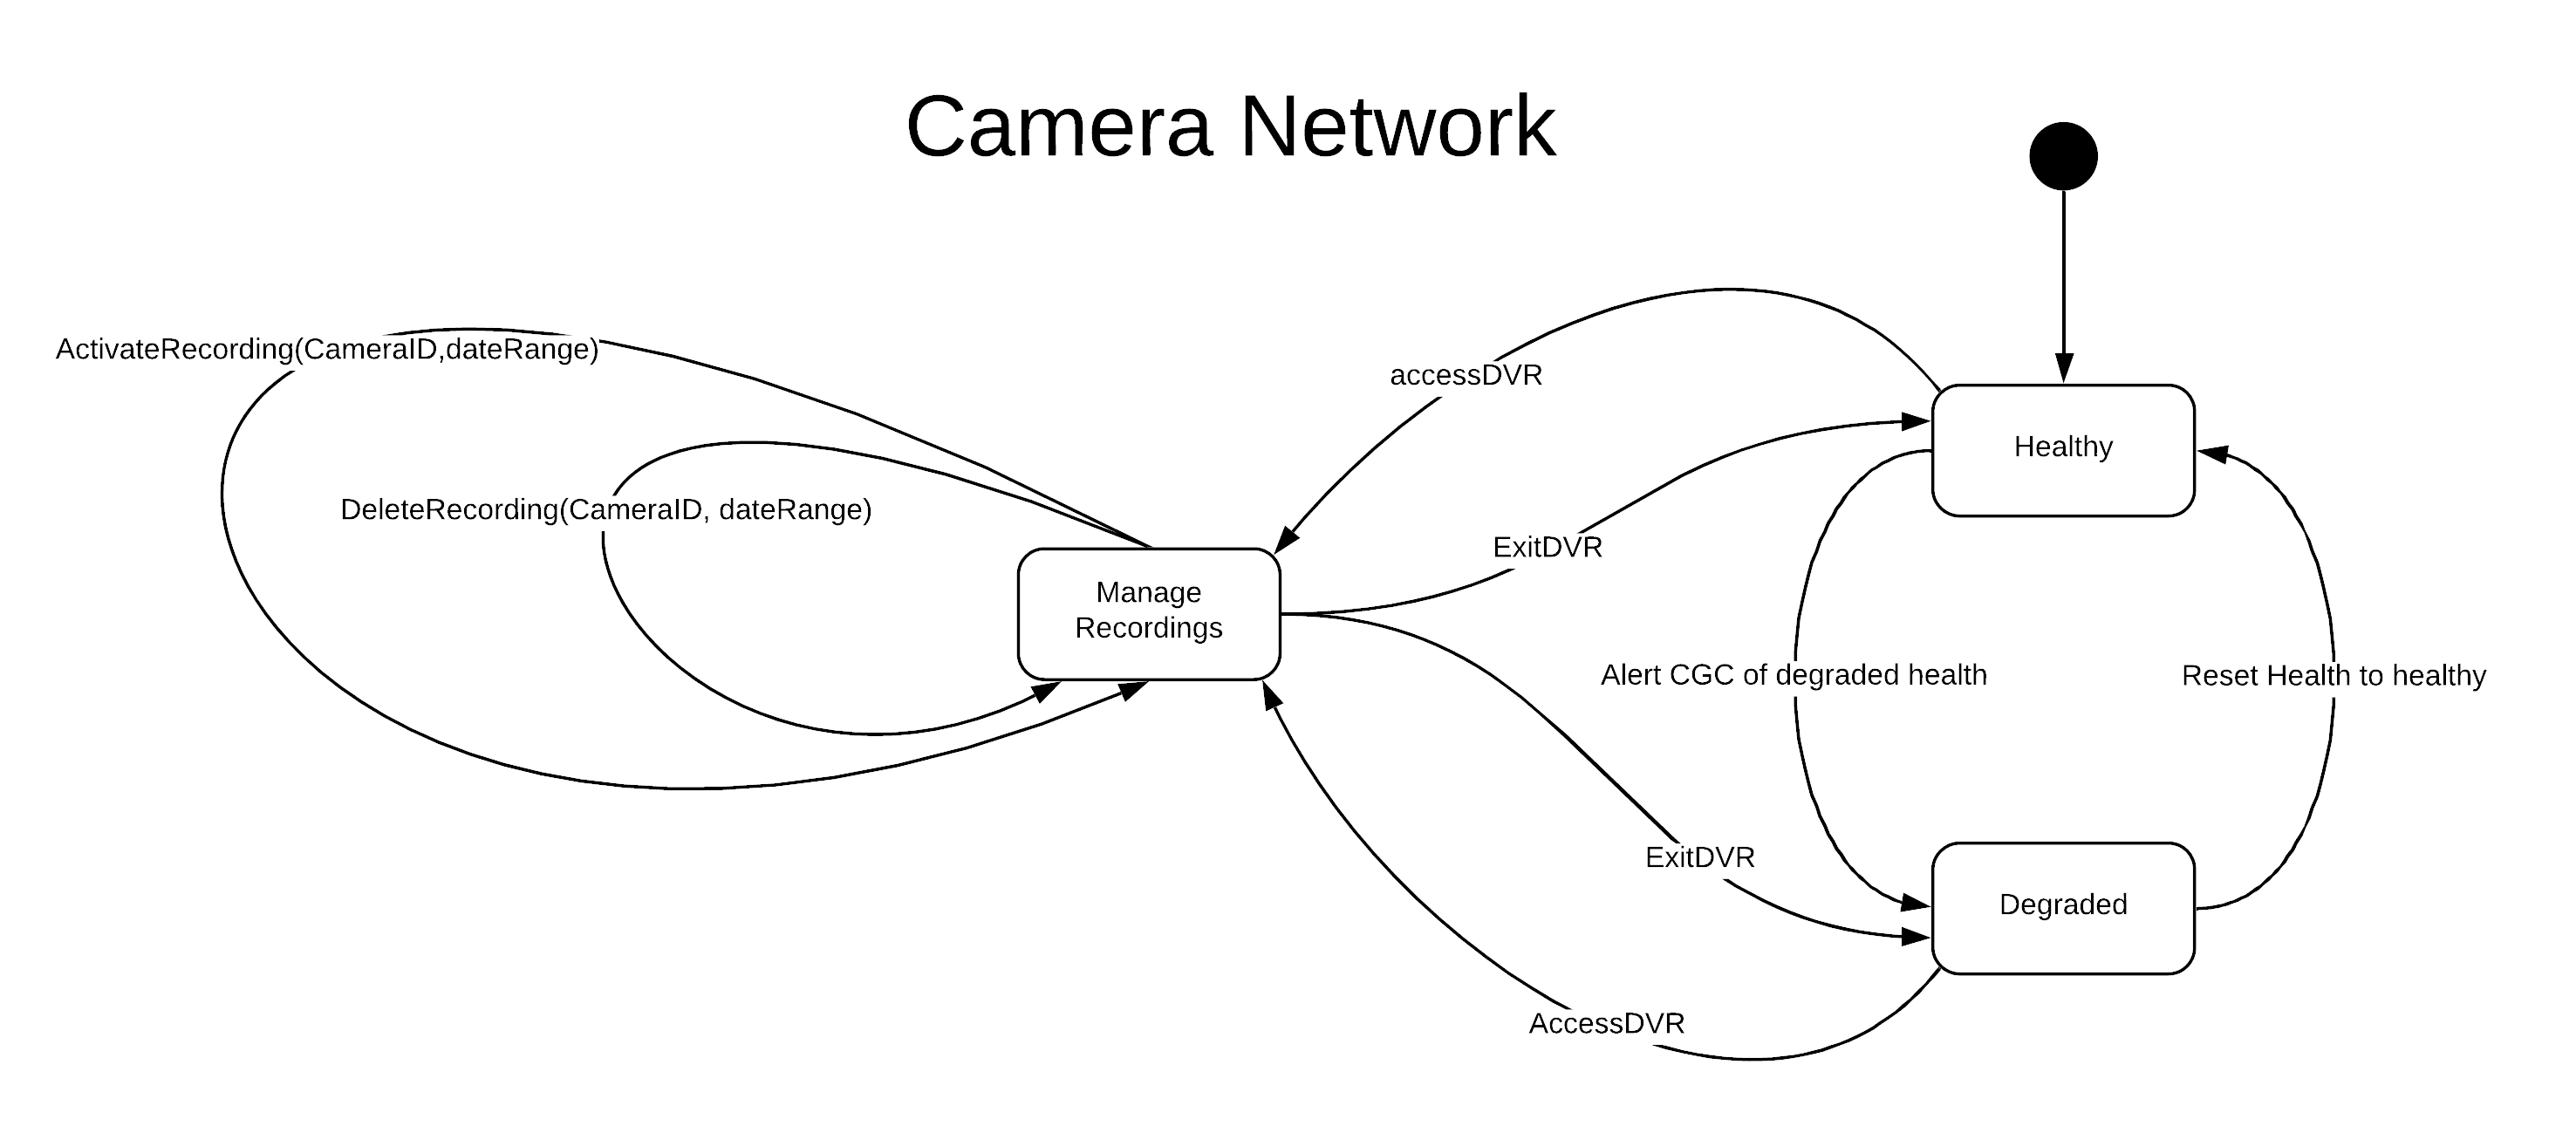
\includegraphics[scale=0.80]{CameraNetwork.png}}
         \caption{Camera Network System Dynamic Control Model}
          \label{fig:cameranetwork}
    \end{figure}

    \paragraph{Electric Fence}
    \paragraph{}\textit{The electric fence can either be in an Idle or healthy state. It could also be in an Emergency state at this point it triggers the entire CGC to go into emergency mode.}
    \begin{figure}[H]
         \centerline{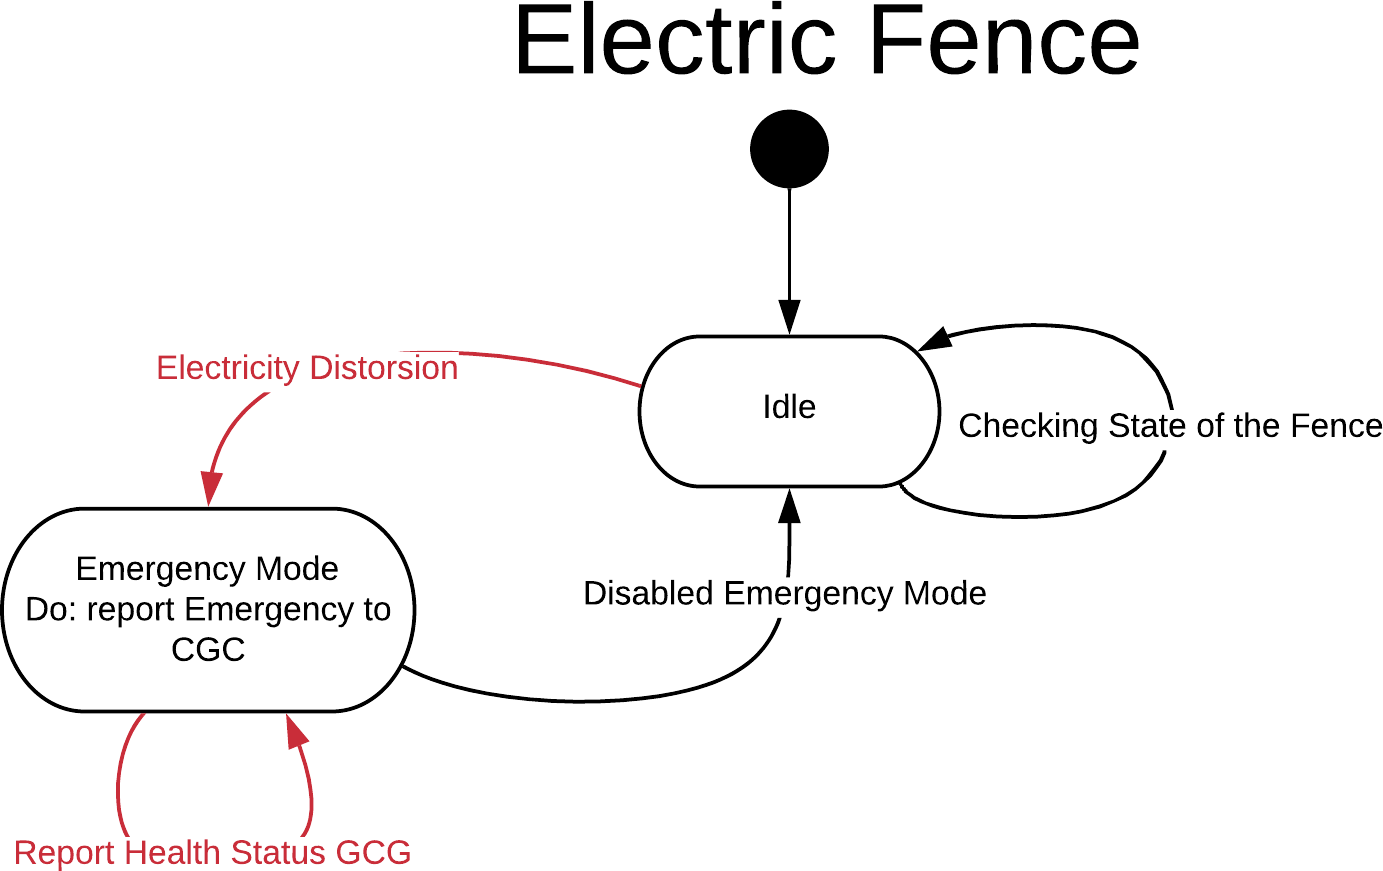
\includegraphics[scale=0.80]{ElectricFence.png}}
         \caption{Electric Fence Dynamic Control Model}
          \label{fig:electricfence}
    \end{figure}

    \paragraph{T-Rex Monitor}
    \paragraph{}\textit{The logic in this diagram is for the T-Rex Monitor}   
    \begin{figure}[H]
         \centerline{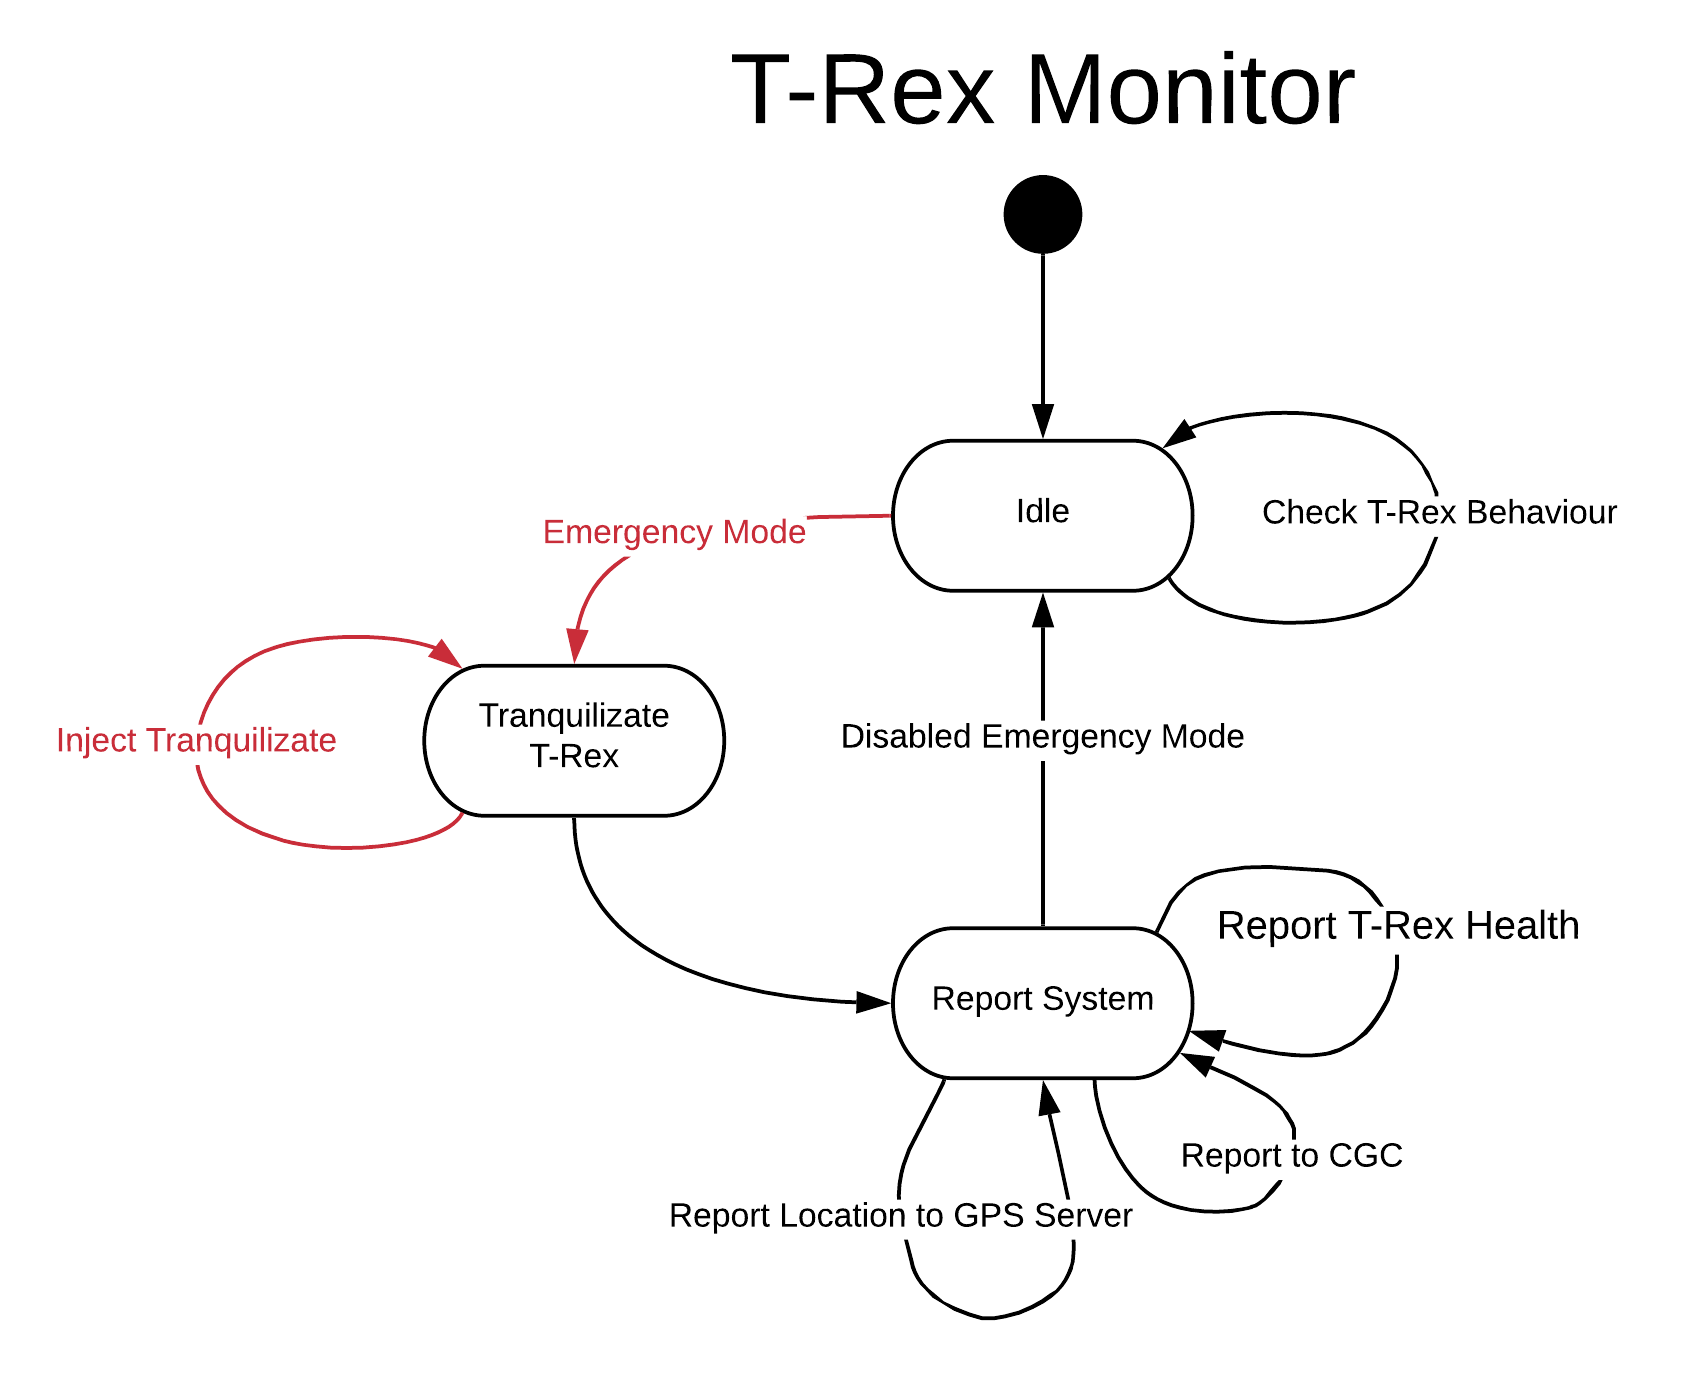
\includegraphics[scale=0.80]{T-RexMonitor.png}}
         \caption{T-Rex Monitor Dynamic Control Model}
          \label{fig:trexmonitor}
    \end{figure}

\section{Design Constraints} \label{cons} 
\paragraph{} \textit{There are quite a bit of constraints\footnote{Design Constraints by Anas Gauba} that the CGC must address in order to successfully function.}

    \subsection{Client}
    \begin{itemize}
        \item The visitors must arrive and purchase tokens from the pay kiosks on the south-end of the island. 
        \item The visitors must get a token which acts as a GPS device as well as RFID key to easily access the perks. 
        \item There must only be one token per visitor.
    \end{itemize}

    \subsection{Safety}
    \begin{itemize}
        \item There must be an emergency mode in the event of the enclosure failure.
        \item The vehicles must alert and instruct visitors in the event of an emergency.
        \item The alarm system must be audible on both the north and south ends.
        \item The vehicles must facilitate evacuation in the event of an emergency.
        \item There must be a surplus of vehicles on either end of the island at all times.
        \item The tokens must provide additional evacuation information such as visitor's location.
        \item The cars must maintain safe speeds at all times.
        \item The cars must lock the doors before moving to its destination.
    \end{itemize}

    \subsection{Regulations}
    \begin{itemize}
        \item The vehicles should accommodate up to ten visitors (excluding the emergency scenario).
        \item The vehicles must alert visitors once their allotted time is up. 
    \end{itemize}

    \subsection{Security}
    \begin{itemize}
        \item The T-Rex location is critical and it must be known at all times.
        \item The camera network stream must be available around the island at all times.
        \item The employee must directly monitor the health of all the devices, especially the ones which can cause harm to the visitors, such as, T-Rex and Electric Fence. 
    \end{itemize}

\section{Sample Use Cases}
\paragraph{} \textit{The CGC lends itself for a substantial amount of uses. Some notable uses include financial,
official, managerial, medical, and technical connotations.}

    \subsection{CGC Station Operator}
    \textit{The CGC Station Operator  (GSO)is the actor responsible for monitoring the central CGC system that
    controls all other components. This individual may communicate with guests or other employees 
    through the car intercom, may place vehicles into manual mode, and has access to the camera network.}
    \par\noindent\rule{\textwidth}{0.4pt}    
    \begin{itemize}
        \item[]\textbf{Use Case:}                                
            ReprimandTroublesomeGuest

        \item[]\textbf{Primary Actor:}
            CGC Station Operator

        \item[]\textbf{Goal in Context:}
            To reprimand a guest that is causing trouble by incremental warnings ranging from
            casual notice, to threats of banishment from the resort.

        \item[]\textbf{Preconditions:}
            The system and all components are functioning properly.

        \item[]\textbf{Trigger:}
            A guest is caught throwing rocks into the enclosure.
            
        \item[]\textbf{Scenario:}
            \begin{enumerate}
                \item The GSO reviews an alert from the electric fence interface.
                \item The GSO reads that small voltage spikes have been detected.
                \item The GSO heads to the surveillance camera that corresponds to the
                panel in question.
                \item The GSO observes a guest hurling rocks at the enclosure, which
                explains the voltage spikes.
                \item The GSO immediately and firmly tells the guest to stop throwing rocks
                through the PA system near the site.
                \item The GSO is ignored by the guest who gives the finger to the camera.
                \item The GSO dispatches the nearest patrol vehicle to the location.
                \item The GSO explains the situation to the security guard that happens 
                to be in the patrol vehicle at the time.
                \item The GSO firmly alerts the unruly guest that a security guard has been sent.
                \item The security guard arrives and reprimands the guest.
                \item The guest become violent and gets tased and pepper sprayed.
                \item The guest is apprehended and placed in the patrol vehicle.
                \item The GSO dismisses the electric fence alerts.
            \end{enumerate}

        \item[]\textbf{Exceptions:}
            \begin{itemize}
                \item[] The system is triggered into emergency mode.
            \end{itemize}

        \item[]\textbf{Priority:}
            Moderate, not necessary, but can be useful.
            
        \item[]\textbf{When Available:}
            On demand.

        \item[]\textbf{Frequency of Use:}
            More frequent with higher volumes of visits.
            
        \item[]\textbf{Channel to Primary Actor:}
            Electric fence panel, CGC Station GUI, camera 

        \item[]\textbf{Secondary Actors:}
            Patrol Vehicle, Security Guard, Electric Fence, Guest
            
        \item[]\textbf{Channels to Secondary Actors:}
            \begin{itemize}
                \item[] Patrol Vehicle: direct
                \item[] Security Guard: car intercom
                \item[] Electric Fence: direct
                \item[] Guest: PA system, electric fence
            \end{itemize}

        \item[]\textbf{Open Issues:}
            \begin{itemize}
                \item[] None known.
            \end{itemize}
    \end{itemize}
     
    \subsection{Emergency Personnel}
    \textit{Emergency Personnel (EP) may be police officers, federal agents, paramedics, and in certain contexts even 
    security guards. Among the many actions that may be taken by such an actor are search and rescue, arrest, perform CPR, 
    and many more.}
    \par\noindent\rule{\textwidth}{0.4pt}    
    \begin{itemize}
        \item[]\textbf{Use Case:}                                
            SearchAndRescue

        \item[]\textbf{Primary Actor:}
            Emergency Personnel

        \item[]\textbf{Goal in Context:}
            To find any potentially remaining guests after a disaster has occurred on the island.
            
        \item[]\textbf{Preconditions:}
            Emergency mode may or may not be currently active, but it has definitely been triggered prior to 
            the arrival of the actor.

        \item[]\textbf{Trigger:}
            A distress signal has been received from Cretaceous Gardens (from Isla Trueno).

        \item[]\textbf{Scenario:}
            \begin{enumerate}
                \item The platoon has received orders to address an emergency on Isla Trueno. 
                \item The troops arrive to the island littered with debris and corpses. 
                \item Some Pay kiosks remain active with an eerie glow coming from an uncannily 
                cheerful welcome screen.
                \item Screams of terror can be heard in the distance, followed by tremendous roars.
                \item The Emergency Personnel head to the kiosks and enter special codes that provide
                them with an enormous supply of token devices.
                \item The EP diffuse throughout the island as they sweep for survivors.
                \item Several helicopters can be heard swarming overhead and small group
                is sent to the CGC Station.
                \item As the troops move inland they find severely injured, but alive, guests.
                \item The troops give the injured new tokens which may be detected by the team
                at the station.
                \item A second group arrives at the island, and is directed by the team at the station
                (via walkie talkies) to the injured.
                \item The team notices the T-Rex Monitor signal moving toward the sweeping group of soldiers
                and they alert them immediately to get into offensive positions.
                \item The helicopters overhead lower themselves to wait for the animal.
                \item Permission to engage is granted and the beast is taken down.
                \item The troops continue their operation until sunrise as teams of paramedics
                are shipped to the island.
            \end{enumerate}

        \item[]\textbf{Exceptions:}
            \begin{itemize}
                \item[] The T.Rex destroys the CGC Station.
            \end{itemize}

        \item[]\textbf{Priority:}
            Essential, must be implemented.
            
        \item[]\textbf{When Available:}
            On demand.

        \item[]\textbf{Frequency of Use:}
            Hopefully never.

        \item[]\textbf{Channel to Primary Actor:}
            Token GPS

        \item[]\textbf{Secondary Actors:}
            Guests, Tokens, Pay Kiosks

        \item[]\textbf{Channels to Secondary Actors:}
            \begin{itemize}
                \item[] Guests: tokens
                \item[] Tokens: pay kiosks
                \item[] Pay Kiosks: direct
            \end{itemize}

        \item[]\textbf{Open Issues:}
            \begin{itemize}
                \item[] None known.
            \end{itemize}
    \end{itemize}
        
    \subsection{Guest}
    \textit{The guest is the primary benefactor of many to the system's features. The primary role of this
    actor is to safely indulge in what the resort has to offer. The most common use for a guest is to see the main
    exhibit but there may be several prerequisite uses that lead up to that.}
    \par\noindent\rule{\textwidth}{0.4pt}    
    \begin{itemize}
        \item[]\textbf{Use Case:}                                
            ViewTRex

        \item[]\textbf{Primary Actor:}
            Guest

        \item[]\textbf{Goal in Context:}
            To see a live dinosaur.

        \item[]\textbf{Preconditions:}
            The system and all components are functioning normally.
            
        \item[]\textbf{Trigger:}
            The guest wishes to see a dinosaur since the age of five.

        \item[]\textbf{Scenario:}
            \begin{enumerate}
                \item Upon hearing of the grand opening of Cretaceous Gardens, the guest immediately
                heads to the island by whatever means possible.
                \item On arrival, the guest witnesses tremendous lines formed at many pay kiosks
                near the entrance of the resort.
                \item After what seems like an eternity, the it is the guest's turn to purchase entry to the resort.
                \item The guest is welcomed through a pleasant graphical display.
                \item The guest is asked a series of questions in order verify compliance with the park policies
                (e.g. How old are you? Do you consent to having your picture taken? Do you accept full responsibility 
                for any injuries sustained due to personal choices? Do you accept the risks of seeing a live 
                Tyrannosaurus Rex and free Cretaceous Gardens of any and all consequences of doing so?)
                \item After ignoring all the fine print and zipping through the legal stuff, the guest finally
                arrives at the screen that will allow the rental of an access token.
                \item The guest enters the amount of time he or she plans to stay and is given the total price.
                \item The guest is prompted to enter payment.
                \item The guest pays after confirmation and receives the rental token device.
                \item Instructions on what to do next are displayed on the kiosk screen.
                \item The guest uses the token device to enter the resort via a small gate.
                \item The guest eventually arrives at a parked car, into which others may or may not be entering.
                \item The guest enters the token device into the seatbelt buckle and secures the seatbelt.
                \item The guest lets the car do its job (see section \ref{carscenarios}).
                \item The guest arrives at the exhibit and exits the car, taking the token device along.
                \item The guest heads toward another gate which scans the token device to provide access.
                \item The guest sprints toward the enclosure.
                \item The guest is lucky and gets to see the mighty T.Rex sniffing around. 
            \end{enumerate}

        \item[]\textbf{Exceptions:}
            \begin{itemize}
                \item[] Guest changes his or her mind anywhere in the scenario and decides to leave.
                \item[] The system is triggered into emergency mode.
            \end{itemize}

        \item[]\textbf{Priority:}
            Essential, must be implemented

        \item[]\textbf{When Available:}
            During business hours.

        \item[]\textbf{Frequency of Use:}
            Up to thousands of times per day
            
        \item[]\textbf{Channel to Primary Actor:}
            External media source, island dock, pay kiosk interface, car door,
            seatbelt buckle, exhibit gate, electric enclosure

        \item[]\textbf{Secondary Actors:}
            Pay Kiosk, Token, Car, T.Rex
            
        \item[]\textbf{Channels to Secondary Actors:}
            \begin{itemize}
                \item[] Pay Kiosk: pay kiosk touch screen, card or cash receptacle, token dispenser
                \item[] Token: token dispenser
                \item[] Car: car door, seatbelt and buckle
                \item[] T.Rex: all the above, and the electric fence enclosure
            \end{itemize}
            
        \item[]\textbf{Open Issues:}
            \begin{itemize}
                \item[] None known.
            \end{itemize}
    \end{itemize}

    \par\noindent\rule{\textwidth}{0.4pt}    
    \begin{itemize}
        \item[]\textbf{Use Case:}                                
            Evacuate

        \item[]\textbf{Primary Actor:}
            Guest

        \item[]\textbf{Goal in Context:}
            To leave the island as quickly and as safely as possible.

        \item[]\textbf{Preconditions:}
            There exists some imminent threat to the guest (it may be an enclosure failure, inclement 
            weather, or any other emergency of similar caliber). Sudden guest death (unrelated to the
            island or system) may also be the case.

        \item[]\textbf{Trigger:}
            Something horrible occurs. For simplicity, the following scenario assumes the T.Rex destroys
            its enclosure and is now on the loose.

        \item[]\textbf{Scenario:}
            \begin{enumerate}
                \item The T.Rex destroys the enclosure (see subsection \ref{trexleave}).
                \item Emergency mode is activated.
                \item22 All guests are alerted via the car intercom, the token devices, and an
                island wide speaker system, the Global Alarm System.
                \item Guests receive instructions via the above means with interleaved reassurances
                that extra vehicles are on the way to pick them up.
                \item Guests are also informed that they may enter any vehicle, with or without tokens.
                \item Once in the vehicle, guests are asked (via the token device) whether or not
                they would like to depart.
                \item If at least one individual submits a yes, the car transmits a message to indicate
                imminent departure with a warning that doors will soon close.
                \item Once in motion, the guest in the driver seat is offered the option to place the vehicle into
                manual mode.
                \item If the individual chooses to do so, then he or she may now pilot the vehicle as he or she wishes.
                \item Otherwise, the car will head south as quickly and as safely as possible.
                \item Once at the south end, the car will park and wait for guests to exit.
                \item After it has been confirmed that no guests remain in the vehicle (seat weight sensors
                indicate all seats are empty), the guests are given another warning to stand back.
                \item As the guests head toward the exit, the car closes its doors and speeds north 
                to collect more guests.
            \end{enumerate}

        \item[]\textbf{Exceptions:}
            \begin{itemize}
                \item[] The car suffers damage that causes it to malfunction.
            \end{itemize}

        \item[]\textbf{Priority:}
            Essential, must be implemented.

        \item[]\textbf{When Available:}
            On demand.

        \item[]\textbf{Frequency of Use:}
            Hopefully never, but at least once in reality.

        \item[]\textbf{Channel to Primary Actor:}
            Car doors, tokens, interior car components (if manual mode is enabled)
            
        \item[]\textbf{Channels to Secondary Actors:}
            \begin{itemize}
                \item[] T.Rex: breached enclosure
                \item[] Token: device display and speaker
                \item[] Emergency Personnel: directly at any stage during the evacuation.
            \end{itemize}
        \item[]\textbf{Secondary Actors:}
            T.Rex, Tokens, Emergency Personnel

        \item[]\textbf{Open Issues:}
            \begin{itemize}
                \item[] None known.
            \end{itemize}
    \end{itemize}
    
    % another use case
    
    % another use case
    
    % ...
    
    \subsection{Guest Vehicle}\label{carscenarios}
    \textit{The guest vehicle (GV) plays a vital role in facilitating the guest experience. The actor primarily
    moves guests to and from the exhibit, but may exhibit other functions when the system is in maintenance or
    emergency mode.}
    \par\noindent\rule{\textwidth}{0.4pt}    
    \begin{itemize}
        \item[]\textbf{Use Case:}                                
            ShuttleGuestsToExhibit

        \item[]\textbf{Primary Actor:}
            Guest Vehicle

        \item[]\textbf{Goal in Context:}
            To transport guests to the northern part of the island so they may 
            visit the exhibit.

        \item[]\textbf{Preconditions:}
            The system is in normal mode and all components are functioning properly.

        \item[]\textbf{Trigger:}
            A transaction is confirmed and a tokens are provided to guests.

        \item[]\textbf{Scenario:}
            \begin{enumerate}
                \item The guests are directed to the parked GV.
                \item The guests enter the GV.
                \item The GV instructs guests to enter their token devices into their belt buckles.
                \item The GV detects all token-containing buckles have been used to fasten corresponding seatbelts.
                \item The GV locks its doors and unlocks window functionality for guests.
                \item The GV performs a quick system check.
                \item The GV heads toward the exhibit.
                \item The GV arrives and parks in front of a gate that leads to the exhibit.
                \item The GV reminds the guests to take their tokens with them as it grants them access through the gate.
                \item The guests exit the vehicle and make their way toward the gate.
                \item The GV parks itself nearby and starts a timer.
            \end{enumerate}

        \item[]\textbf{Exceptions:}
            \begin{itemize}
                \item[] A guest loses his or her token device, thus preventing seatbelt access, which necessitates
                staff intervention.
            \end{itemize}

        \item[]\textbf{Priority:}
            Essential, must be implemented.

        \item[]\textbf{When Available:}
            On Demand.

        \item[]\textbf{Frequency of Use:}
            Up to thousands of times per day.
            
        \item[]\textbf{Channel to Primary Actor:}
            Direct.

        \item[]\textbf{Secondary Actors:}
            Guests, CGC Station Operator, Tokens
            
        \item[]\textbf{Channels to Secondary Actors:}
            \begin{itemize}
                \item[] Guests: doors, seatbelts, speakers
                \item[] CGC Station Operator: direct
                \item[] Tokens: seatbelt buckles
            \end{itemize}

        \item[]\textbf{Open Issues:}
            \begin{itemize}
                \item[] None known.
            \end{itemize}
    \end{itemize}

    \par\noindent\rule{\textwidth}{0.4pt}    
    \begin{itemize}
        \item[]\textbf{Use Case:}                                
            ShuttleGuestsFromExhibit

        \item[]\textbf{Primary Actor:}
            Guest Vehicle

        \item[]\textbf{Goal in Context:}
            To transport guests to the southern part of the island so they may 
            leave the island.

        \item[]\textbf{Preconditions:}
            The system is in normal mode and all components are functioning properly.

        \item[]\textbf{Trigger:}
            The guests' time is up at the exhibit.

        \item[]\textbf{Scenario:}
            \begin{enumerate}
                \item The car alerts the guests it shuttled to the exhibit that time is up.
                \item The guests hear the alert from the car and from their token devices.
                \item Some of the guests immediately head to the car while others delay.
                \item The guests that head to the car enter it and fasten their seat belts.
                \item The GV sends another alert to those remaining.
                \item The rest of the guests finally arrive and enter the GV.
                \item The GV locks its doors after everyone has fastened their seatbelts.
                \item The GV heads south.
                \item The GV arrives to the southern part of the island where it parks.
                \item The guests release their seatbelts.
                \item The GV unlocks its doors and allows the guests to exit.
                \item The GV is dispatched elsewhere.
            \end{enumerate}

        \item[]\textbf{Exceptions:}
            \begin{itemize}
                \item[] A guest happens to be injured and requires another type of transportation.
                \item[] A guest loses his or her token device, thus preventing seatbelt access.
            \end{itemize}

        \item[]\textbf{Priority:}
            Essential, must be implemented.

        \item[]\textbf{When Available:}
            On Demand.

        \item[]\textbf{Frequency of Use:}
            Up to thousands of times per day.
            
        \item[]\textbf{Channel to Primary Actor:}
            Direct.

        \item[]\textbf{Secondary Actors:}
            Guests, CGC Station Operator, Tokens
            
        \item[]\textbf{Channels to Secondary Actors:}
            \begin{itemize}
                \item[] Guests: doors, seatbelts, speakers
                \item[] CGC Station Operator: direct
                \item[] Tokens: seatbelt buckles
            \end{itemize}

        \item[]\textbf{Open Issues:}
            \begin{itemize}
                \item[] None known.
            \end{itemize}
    \end{itemize}
    
    \subsection{Maintenance Personnel}
    \textit{Maintenance Personnel (MP) is responsible for the physical connections 
    and addressing any issues with the physical components used with by the CGC (e.g cameras, 
    kiosks, cars, enclosure panels, etc.). This individual would be in charge of responding to nodal failures.}
    \par\noindent\rule{\textwidth}{0.4pt}    
    \begin{itemize}
        \item[]\textbf{Use Case:}                                
            RepairExternalEnclosureCamera

        \item[]\textbf{Primary Actor:}
            Network Maintenance Personnel

        \item[]\textbf{Goal in Context:}
            To fix or replace a malfunctioning or broken camera that has been detected to
            be in such a state by the CGC. The camera in question resides outside the exhibit
            enclosure.

        \item[]\textbf{Preconditions:}
            The CGC is not in emergency mode but may be in either normal or maintenance mode, and
            the issue has already been diagnosed (i.e. it is known with certainty that the problem
            is the camera and not the link to the camera).

        \item[]\textbf{Trigger:}
            The CGC reports an error in some camera within the Camera Network after 
            failing to make contact via alternate paths.

        \item[]\textbf{Scenario:}
            \begin{enumerate}
                \item NMP is dispatched and transported in an self-driving car to the 
                location of the problem by the CGC Station Operator (CSO).
                \item NMP arrives and performs a repair, exchanges the broken camera
                for a new one, or attaches a new one if it happens to be gone all together.
                \item The CSO and NMP perform tests to ensure proper function.
                \item The maintenance is concluded.
                \item The NMP is dispatched to any other components that may need servicing.
                \item [OR]
                \item The NMP returns any removed parts (e.g. the broken camera) to a stock room.
            \end{enumerate}

        \item[]\textbf{Exceptions:}
            \begin{itemize}
                \item[] Maintenance materials are out of stock.
                \item[] Emergency mode interrupts the procedure.
            \end{itemize}

        \item[]\textbf{Priority:}
            Moderate, should be implemented.

        \item[]\textbf{When Available:}
            On Demand.

        \item[]\textbf{Frequency of Use:}
            It may vary with respect to the average lifetime of the cameras in the network.

        \item[]\textbf{Channel to Primary Actor:}
            CGC Station, Car, Camera, Camera Network

        \item[]\textbf{Secondary Actors:}
            CGC Station Operator, Camera Network
            
        \item[]\textbf{Channels to Secondary Actors:}
            \begin{itemize}
                \item[] CGC Station Operator: Car Intercom
                \item[] Camera Network: Camera
            \end{itemize}

        \item[]\textbf{Open Issues:}
            \begin{itemize}
                \item[] None known
            \end{itemize}
    \end{itemize}
%    
%    % another use case
%    
%    % another use case
%    
%    % ...
    
    \subsection{Patrol Vehicle}
    \textit{This actor is a special type of autonomous vehicle that patrols the island for an 
    added layer of protection and in the interest of guest welfare.}
    \par\noindent\rule{\textwidth}{0.4pt}    
    \begin{itemize}
        \item[]\textbf{Use Case:}                                
            PatrolIsland

        \item[]\textbf{Primary Actor:}
            Patrol Vehicle

        \item[]\textbf{Goal in Context:}
            To provide a means via which security personnel may patrol the island. The vehicles
            are to be on a mostly predetermined route, so the security guards (in this context)
            are mostly passive agents.

        \item[]\textbf{Preconditions:}
            The system is in normal mode and all components are functioning properly.

        \item[]\textbf{Trigger:}
            The resort opens for business.

        \item[]\textbf{Scenario:}
            \begin{enumerate}
                \item Cretaceous Gardens opens to employees before opening for the business day.
                \item The Patrol Vehicle (PV) is dispatched via a routine protocol.
                \item The PV performs a test run around the island before picking up the security guard
                of the shift.
                \item The security guard enters the PV, after which the PV performs another test trip.
                \item The security guard double checks state of the route.
                \item Anything out of the ordinary is reported to the relevant parties (maintenance for example).
                \item The PV returns to the southern part of the island.
                \item The security guard confirms an all clear with other employees.
                \item The rest of the employees continue their setup as the security guard enters the PV.
                \item The PV begins its daily patrolling routine (one or more simple circuits around the island).
            \end{enumerate}

        \item[]\textbf{Exceptions:}
            \begin{itemize}
                \item[] The system is triggered into emergency mode.
            \end{itemize}

        \item[]\textbf{Priority:}
            Low, not necessary but may be useful.

        \item[]\textbf{When Available:}
            During business hours.

        \item[]\textbf{Frequency of Use:}
            Daily.

        \item[]\textbf{Channel to Primary Actor:}
            Direct.

        \item[]\textbf{Secondary Actors:}
            CGC Station Operator, Security Guard
            
        \item[]\textbf{Channels to Secondary Actors:}
            \begin{itemize}
                \item[] Security Guard: Car door, inner components of car 
                \item[] CGC Station Operator: CGC station interface
            \end{itemize}

        \item[]\textbf{Open Issues:}
            \begin{itemize}
                \item[] None known.
            \end{itemize}
    \end{itemize}
%    
%    % another use case
%    
%    % another use case
%    
%    % ...

    \subsection{Sales department}
    \textit{The sales department (SD) is, for the sake of simplicity, is the actor interested 
    in maximizing ticket sales and profits. The SD is interested in any financial trends
    for the sake of such aims. They may also be interested in finding efficiency bottle necks
    that incur unnecessary costs.}
    \par\noindent\rule{\textwidth}{0.4pt}    
    \begin{itemize}
        \item[]\textbf{Use Case:}                                
            VisualizeSalesData

        \item[]\textbf{Primary Actor:}
            Sale Department

        \item[]\textbf{Goal in Context:}
            To acquire and study data related to sales within some given period of time.

        \item[]\textbf{Preconditions:}
            The system is not in emergency mode nor maintenance mode and all components are 
            functioning properly.

        \item[]\textbf{Trigger:}
            It is about time to wrap up a fiscal quarter to plan for the next one.

        \item[]\textbf{Scenario:}
            \begin{enumerate}
                \item A meeting is scheduled in order to plan for the next quarter.
                \item The SD gathers all sales data provided by the CGC.
                \item The SD uses a provided interface to organize the data into meaningful visualizations.
                \item The SD exports the visualizations for a presentation at the meeting.
                \item The meeting is held and the SD presents their findings.
                \item The SD contribution helps guide the conversation for what to do next.
                \item The meeting concludes. 
            \end{enumerate}

        \item[]\textbf{Exceptions:}
            \begin{itemize}
                \item[] The system enter emergency mode.
            \end{itemize}

        \item[]\textbf{Priority:}
            Extremely low, need not be implemented.

        \item[]\textbf{When Available:}
            On demand.

        \item[]\textbf{Frequency of Use:}
            May be used continuously (as a live data feed), or any number of snapshots
            may be taken hourly, daily, weekly, etc.

        \item[]\textbf{Channel to Primary Actor:}
            An auxiliary interface specialized for financial data visualization.

        \item[]\textbf{Secondary Actors:}
            CGC Control Station
            
        \item[]\textbf{Channels to Secondary Actors:}
            \begin{itemize}
                \item[] CGC Control Station: some network link to forward relevant data
            \end{itemize}

        \item[]\textbf{Open Issues:}
            \begin{itemize}
                \item[] An interface separate from the Control Station interface would have to
                be developed as it would reside elsewhere on the island.
            \end{itemize}
    \end{itemize}
    
    % another use case
    
    % another use case
    
    % ...

%%%%% Siri %%%%%
    \subsection{System Administrator}
    \textit{The this actor (SA) specializes in addressing hardware issues with the CGC Station. This
    individual is responsible for repairing disk drives, monitors, redundancy elements within the
    station, updating machine operating systems, etc.}
    \par\noindent\rule{\textwidth}{0.4pt}    
    \begin{itemize}
        \item[]\textbf{Use Case:}                                
            UpgradeSystemMemory

        \item[]\textbf{Primary Actor:}
            CGC System Technician

        \item[]\textbf{Goal in Context:}
            To upgrade the memory of the machines within at CGC Control Station (e.g. add 16 GB RAM).

        \item[]\textbf{Preconditions:}
            The CGC is not in emergency mode but may be in either maintenance or normal mode.

        \item[]\textbf{Trigger:}
            Cretaceous Gardens experiences an increase in demand, which (if the trend continues) will
            require more computational resources to handle more guests, more efficiently.

        \item[]\textbf{Scenario:}
            \begin{enumerate}
                \item The Sales Department notices a distinct upward trend in sales.
                \item The findings percolate through the relevant business entities within the company.
                \item The CST is dispatched to the Control Station.
                \item The CST enables maintenance mode.
                \item The CST upgrades machines that are currently being used for redundancy.
                \item The CST enables maintenance mode on the redundant machines.
                \item The redundant machines and active machines, switch roles.
                \item The CST upgrades the now-redundant machines.
                \item The CST performs tests.
                \item The CST disables maintenance mode in both active, and redundant machines.
            \end{enumerate}

        \item[]\textbf{Exceptions:}
            \begin{itemize}
                \item[] The trend is ignored by management.
            \end{itemize}

        \item[]\textbf{Priority:}
            Moderate, should be implemented.

        \item[]\textbf{When Available:}
            On demand.

        \item[]\textbf{Frequency of Use:}
            Every two or three fiscal years.

        \item[]\textbf{Channel to Primary Actor:}
            Control station hardware.
        
        \item[]\textbf{Secondary Actors:}
            Sales Department, CGC Control Station, Pay Kiosk
                
        \item[]\textbf{Channels to Secondary Actors:}
            \begin{itemize}
                \item[] Sales Department: pay kiosk transaction logs
                \item[] CGC Control Station: direct access
                \item[] Pay Kiosk: direct connection
            \end{itemize}

        \item[]\textbf{Open Issues:}
            \begin{itemize}
                \item[] None known.
            \end{itemize}
    \end{itemize}
    
    \subsection{System Auditor}
    \textit{This actor (SA) may be an external individual that may either be hired by Cretaceous 
    Gardens to test the robustness of the system, or whose inspection may be mandated by law.}
    \par\noindent\rule{\textwidth}{0.4pt}    
    \begin{itemize}
        \item[]\textbf{Use Case:}                                
            SimulateProtocols

        \item[]\textbf{Primary Actor:}
            System Auditor

        \item[]\textbf{Goal in Context:}
            To observe currently implemented protocols within the system and provide an analysis
            regarding their safety.

        \item[]\textbf{Preconditions:}
            The system is not in emergency mode nor maintenance mode, but may be put into such
            modes for testing purposes (presumably outside business hours).

        \item[]\textbf{Trigger:}
            The time for a system audit has arrived, either after being scheduled or at random.

        \item[]\textbf{Scenario:}
            \begin{enumerate}
                \item The SA arrives to the CGC Control Station outside of business hours.
                \item The SA requests to observe a simulation of the currently used functions of the system.
                \item The SA is provided with a set of protocols that may be simulated.
                \item For each protocol, the SA runs a simulation.
                \item The system passes the audit and the SA leaves.
                \item OR
                \item The system fails while simulating one or more protocols and the auditor presents a deadline
                to fix the issue lest a fine is incurred.
            \end{enumerate}

        \item[]\textbf{Exceptions:}
            \begin{itemize}
                \item[] An audit occurs in the middle of a system upgrade.
                \item[] The system is triggered into emergency mode (due to an actual emergency)
            \end{itemize}

        \item[]\textbf{Priority:}
            Low, not explicitly required, but may be useful for legal robustness.

        \item[]\textbf{When Available:}
            On demand.

        \item[]\textbf{Frequency of Use:}
            Annually or less frequently.

        \item[]\textbf{Channel to Primary Actor:}
            CGC Control Station interface

        \item[]\textbf{Secondary Actors:}
            CGC Control Station, Pay Kiosks, Cars, Electric Fence, T.Rex, 
            T.Rex Monitor, Camera Network
            
        \item[]\textbf{Channels to Secondary Actors:}
            \begin{itemize}
                \item[] CGC Control Station: simulation
                \item[] Pay Kiosks: simulation
                \item[] Cars: simulation
                \item[] Electric Fence: simulation
                \item[] T.Rex: simulation
                \item[] T.Rex Monitor: simulation
                \item[] Camera Network: simulation
            \end{itemize}

        \item[]\textbf{Open Issues:}
            \begin{itemize}
                \item[] What factors should be relevant in a simulation?
            \end{itemize}
    \end{itemize}

    % another use case
    
    % another use case
    
    % ...
    

%%%%% Zeke %%%%%
    \subsection{Tyrannosaurus Rex}\label{trexleave}
    \textit{It may be argued that this is not a legitimate actor, but despite its unconscious interaction
    with the system, the T.Rex can act on the system in a variety of - possibly unpredictable - ways.}
    \par\noindent\rule{\textwidth}{0.4pt}    
    \begin{itemize}
        \item[]\textbf{Use Case:}
            LeaveEnclosure

        \item[]\textbf{Primary Actor:}
            T.Rex

        \item[]\textbf{Goal in Context:}
            To get somewhere that happens to be outside the enclosure.

        \item[]\textbf{Preconditions:}
            Actor is not sedated, the system is not in maintenance mode 
            nor emergency mode, and all components are functioning properly.

        \item[]\textbf{Trigger:}
            The T.Rex sees or smells something outside the enclosure.

        \item[]\textbf{Scenario:}                    
            \begin{enumerate}
                \item The actor looks through the enclosure, 
                toward an imagined near-future destination beyond
                the enclosure. \label{beginTRLeave}
                \item The actor walks toward the target destination.
                \item The actor is impeded by the electric fence. \label{impedeTRLeave}
                \item The actor becomes fearful.
                \begin{enumerate}
                    \item The actor retreats from the fence.
                    \item[OR]
                    \item The actor attacks the fence. 
                \end{enumerate}
                \item The electric fence increases its voltage.
                \item The scenario may repeat from either 
                act \ref{beginTRLeave}, from act \ref{impedeTRLeave}, 
                or continues such that:
                \begin{enumerate}
                    \item the actor is sedated to prevent further damage
                    to self or enclosure, and maintenance mode is triggered
                    \item[OR]
                    \item the enclosure is breached, the actor 
                    heads toward the target destination, and emergency
                    mode is triggered.
                    \item[OR]
                    \item the actor relinquishes the desire to head
                    toward the target destination, no significant damage
                    is incurred, and the normal mode of operation continues.
                \end{enumerate} 
            \end{enumerate}

        \item[]\textbf{Exceptions:}
            \begin{itemize}
                \item[] Actor Perishes.
            \end{itemize}

        \item[]\textbf{Priority:}
            Essential, must be implemented.

        \item[]\textbf{When Available:}
            At random.

        \item[]\textbf{Frequency of Use:}
            Preferably never, but less likely with time (ideally)

        \item[]\textbf{Channels to Primary Actor:}
            \begin{itemize}
                \item[] Electric Enclosure Panel
                \item[] T.Rex Monitor
            \end{itemize}
            
        \item[]\textbf{Secondary Actors:}
            CGC Station Operator, Global Alarm System
            
        \item[]\textbf{Channels to Secondary Actors:}  
            \begin{itemize}
                \item[] CGC Station Operator: Camera Network, T.Rex Monitor
                \item[] Global Alarm System: Electric Enclosure Panel
            \end{itemize}

        \item[]\textbf{Open Issues:}
            \begin{itemize}
                \item[] None known.
            \end{itemize}
    \end{itemize}
    
    % another use case
    
    % another use case
    
    % ...
    
    \subsection{Veterinarian}
    \textit{The veterinarian role includes uses such as routine checkups or medical treatment for the T.Rex.}
    \par\noindent\rule{\textwidth}{0.4pt}    
    \begin{itemize}
        \item[]\textbf{Use Case:}                                
            RoutineCheckup

        \item[]\textbf{Primary Actor:}
            Veterinarian

        \item[]\textbf{Goal in Context:}
            To perform a regular physical exam on the T.Rex.

        \item[]\textbf{Preconditions:}
            The T.Rex has been successfully sedated, the veterinarian is completely prepared, 
            the CGC is not in emergency mode, and all components are functioning properly.

        \item[]\textbf{Trigger:}
            The time for a physical has arrived.

        \item[]\textbf{Scenario:}
            \begin{enumerate}
                \item The CGC Station Operator dispatches the veterinarian in a self driving car
                to the edge of the enclosure closest to the current location of the T.Rex.
                \item The veterinarian requests an all-clear confirmation from the operator.
                \item The CGC Station Operator confirms sedated state of the T.Rex.
                \item The operator disengages the electricity of the panel to provide access.
                \item The veterinarian enters and travels toward the animal.
                \item The operator starts a timer.
                \item The veterinarian arrives at the location of the animal.
                \item The operator stops the timer. 
                \item The veterinarian performs a physical exam while the operator provided updates
                on the sedative state of the T.Rex.
                \item The operator alerts the veterinarian when the previously recorded elapsed time
                is approaching the approximated amount of time until the T.Rex wakes up.
                \item The veterinarian concludes the exam.
                \item The veterinarian replenishes the sedative reservoir in the T.Rex Monitor.
                \item The veterinarian travels toward the point of entry.
                \item The veterinarian exits the enclosure.
                \item The Operator confirms successful exit.
                \item The Operator reengages the electricity of the panel.                 
            \end{enumerate}

        \item[]\textbf{Exceptions:}
            \begin{itemize}
                \item[] The T.Rex is found to be in poor health.
                \item[] The sedative lasts less time than expected.
            \end{itemize}

        \item[]\textbf{Priority:}
            Essential, must be implemented.

        \item[]\textbf{When Available:}
            On Demand.

        \item[]\textbf{Frequency of Use:}
            As little as once a year.

        \item[]\textbf{Channel to Primary Actor:}
            \begin{itemize}
                \item[] Enclosure Panel, T.Rex Monitor
            \end{itemize}

        \item[]\textbf{Secondary Actors:}
            CGC Station Operator, T.Rex, Car
        
        \item[]\textbf{Channels to Secondary Actors:}
            \begin{itemize}
                \item[] CGC Station Operator: Car Intercom, Camera Network
                \item[] T.Rex: Enclosure Panel, T.Rex Monitor
            \end{itemize}

        \item[]\textbf{Open Issues:}
            \begin{itemize}
                \item[] Should the panel remain inactive while 
                the veterinarian is inside?
                \item[] Should the veterinarian simply wear an electric 
                safety suit to avoid disengagement all together?
            \end{itemize}
    \end{itemize}
    
    % another use case
    
    % another use case
    
    % ...
    
    \subsection{Zookeeper} \label{zook}
    \textit{A zookeeper may interact with the CGC in a variety of ways, but some of the
    major roles of such an actor (as with any zookeeper) are to prepare the diet of the T-Rex, 
    feed the T.Rex, to observe its behavior, or groom it.}
    \par\noindent\rule{\textwidth}{0.4pt}    
    \begin{itemize}
        \item[]\textbf{Use Case:} 
            FeedTRex                                

        \item[]\textbf{Primary Actor:}
            Zookeeper

        \item[]\textbf{Goal in Context:}
            To safely provide food for the T.Rex, whether it be live, frozen, thawed, or prepared
            prey.

        \item[]\textbf{Preconditions:}
            The CGC is not in emergency mode, and all components are fully functional.

        \item[]\textbf{Trigger:}
            It is time to feed the T.Rex.

        \item[]\textbf{Scenario:}
            \begin{enumerate}
                \item The CGC Station Operator dispatches the zookeeper in a self driving car
                to the edge of the enclosure furthest from the current location of the T.Rex.
                \item The Zookeeper requests an all-clear confirmation from the operator.
                \item The operator disengages the electricity of the panel to provide access.
                \item The Zookeeper enters and travels a significant distance into the enclosure.
                \item The Zookeeper drops off the food.
                \item The Zookeeper travels back the point of entry.
                \item The Zookeeper exits the enclosure.
                \item The Operator confirms successful exit.
                \item The Operator reengages the electricity of the panel. 
            \end{enumerate}

        \item[]\textbf{Exceptions:}
            \begin{itemize}
                \item[] There is a shortage of food on the island.
                \item[] The T.Rex is sick or injured and does not want to eat.
                \item[] The T.Rex reaches the zookeeper before the zookeeper exits the enclosure.
            \end{itemize}

        \item[]\textbf{Priority:}
            Essential, must be implemented

        \item[]\textbf{When Available:}
            On demand and via operator-zookeeper protocol

        \item[]\textbf{Frequency of Use:}
            Periodically (it can be daily, weekly, or monthly for example)

        \item[]\textbf{Channel to Primary Actor:}
            \begin{itemize}
                \item[] Enclosure Panel
            \end{itemize}

        \item[]\textbf{Secondary Actors:}
            CGC Station Operator, T.Rex, Car
        
        \item[]\textbf{Channels to Secondary Actors:}
            \begin{itemize}
                \item[] CGC Station Operator: Car Intercom, Camera Network
                \item[] T.Rex: Enclosure Panel
            \end{itemize}

        \item[]\textbf{Open Issues:}
            \begin{itemize}
                \item[] Should the panel remain inactive while 
                the zookeeper is inside?
                \item[] Should the zookeeper simply wear an electric 
                safety suit to avoid disengagement all together?
            \end{itemize}
    \end{itemize}
    
    % another use case
    
    % another use case
    
    % ...
    

% secondary actors (note that primary actors above may be secondary in some contexts)
% any devices not mentioned above
% any humans not mentioned above


\section{Definition of Terms} \label{defs}
    \paragraph{} \textit{The following is a list of definitions \footnote{Definition of 
    Terms by Anas Gauba} of the most commonly used technical terms within this 
    document, whose meaning may not be immediately apparent to the lay reader. Most 
    definitions come from no specific source; instead they are defined by the authors 
    in the context of their use in this document and originate from the vocabulary 
    shared across the general references cited \nocite{*}. In the event that a 
    definition was taken directly from a source, it is followed by a citation}
    
    \begin{list}{}{}
        \item \textbf{CGC:} Acronym for Cretaceous Gardens Controller 
        \item \textbf{DVR:} Acronym for Digital Video Recorder
        \item \textbf{Electrical Conduction:} The movement of electrically charged     
            particles through a transmission medium.
        \item \textbf{GPS:} Global Positioning System 
        \item \textbf{Hardwired Ethernet:} This references the latest IEEE standard for 
            Ethernet utilizing physical cables.
        \item \textbf{Network:} All nodes with which the CGC interacts, the links that 
            connect them to each other and to the
            CGC, the CGC itself, and all related databases.
        \item \textbf{Node:} The generic term that refers to any device connected to 
            the CGC in any way. This includes 
            autonomous vehicles, tokens, the T.Rex monitor, all electric fence panels, 
            all kiosks, and all cameras.
        \item \textbf{Safely Inactive:} A state in which a vehicle is fully functional 
            and ready to be dispatched.
        \item \textbf{Safely Occupied:} A state in which a vehicle contains at least 
            one person, is locked, and is ready to depart.
        \item \textbf{Token:} An interactive device used by the visitor that grants 
            access to locations.
    \end{list}
\pagebreak
\bibliography{../../ReferenceMaterial/BibTeX/references}
% run latex, then bibtex, then quickbuild (on the tex file)
\end{document}
